% Robert Gorrie, 2017
%
% Thesis Template By:
%
% Kartik Singhal
% BTech CSE Batch of 2009-13
% NIT Calicut
% Contact Info: kartiksinghal@gmail.com
%
% Released under Creative Commons Attribution license (CC-BY)
% Info: http://creativecommons.org/licenses/by/3.0/

\documentclass[12pt,a4paper]{report}

\usepackage[pdftex]{graphicx}        %for embedding images
\usepackage{xcolor}                  %for colouring in math mode
\usepackage{url}                     %for proper url entries
\usepackage{listings}                %for writing c code
%\usepackage{hyperref}
\usepackage{amssymb}                 %extended symbols
\usepackage{amsthm}                  %theorem formatting
\usepackage{amsmath}                 %misc math formatting
\usepackage{algorithm}
\usepackage{booktabs}                %for toprule, midrule, etc
\usepackage[margin=1in]{geometry}
\usepackage[noend]{algpseudocode}
\usepackage{mathtools}
\usepackage{tikz}
\usepackage{pgfplots}
\usepackage{tcolorbox}
\usepackage{xspace}
\usepackage{enumitem}
\usepackage[toc,page]{appendix}

%for editing purposes
%\usepackage{setspace}
%\doublespacing
%%%%%%%%%%%%%%%%%%%%

\usepackage[bookmarks, colorlinks=false, pdfborder={0 0 0}, pdftitle={title goes here}, pdfauthor={Robert W.V. Gorrie}, pdfsubject={<subject here>}, pdfkeywords={<keywords here>}]{hyperref} %for creating links in the pdf version and other additional pdf attributes, no effect on the printed document

\usetikzlibrary{intersections,decorations.markings,matrix,calc,positioning,decorations.pathreplacing}

\newcommand{\commentblock}[1]{}            %command for multiline comments for testing purposes

\theoremstyle{theorem}
\newtheorem{theorem}{Theorem}
\newtheorem{lemma}{Lemma}
\theoremstyle{definition}
\newtheorem{definition}{Definition}

\tcbset{colback=white!5!white,colframe=black!75!black} %style for theorem and definition boxes

%shortcuts for colour-coded curve parameters for alice
\newcommand{\alice}[0]{\textcolor{red}{Alice}\xspace}
\newcommand{\ba}[0]{\textcolor{red}{A}\xspace}
\newcommand{\laea}[0]{\textcolor{red}{\ell_{A}^{e_A}}}
\newcommand{\la}[0]{\textcolor{red}{\ell_{A}}}
\newcommand{\ea}[0]{\textcolor{red}{e_A}}
\newcommand{\pa}[0]{\textcolor{red}{\phi_A}}
\newcommand{\pap}[0]{\textcolor{red}{\phi'_A}}
\newcommand{\agens}[0]{\{\textcolor{red}{P_A},\textcolor{red}{Q_A}\}}
\newcommand{\genpa}[0]{\textcolor{red}{P_A}}
\newcommand{\genqa}[0]{\textcolor{red}{Q_A}}
\newcommand{\ma}[0]{\textcolor{red}{m_A}}
\newcommand{\na}[0]{\textcolor{red}{n_A}}
\newcommand{\ska}[0]{\textcolor{red}{sk_A}}
\newcommand{\pka}[0]{\textcolor{red}{pk_A}}
%shortcuts for colour-coded curve parameters for bob
\newcommand{\bob}[0]{\textcolor{blue}{Bob}\xspace}
\newcommand{\rb}[0]{\textcolor{blue}{B}\xspace}
\newcommand{\lbeb}[0]{\textcolor{blue}{\ell_{B}^{e_B}}}
\newcommand{\lb}[0]{\textcolor{blue}{\ell_{B}}}
\newcommand{\eb}[0]{\textcolor{blue}{e_B}}
\newcommand{\pb}[0]{\textcolor{blue}{\phi_B}}
\newcommand{\pbp}[0]{\textcolor{blue}{\phi'_B}}
\newcommand{\bgens}[0]{\{\textcolor{blue}{P_B},\textcolor{blue}{Q_B}\}}
\newcommand{\genpb}[0]{\textcolor{blue}{P_B}}
\newcommand{\genqb}[0]{\textcolor{blue}{Q_B}}
\newcommand{\mb}[0]{\textcolor{blue}{m_B}}
\newcommand{\nb}[0]{\textcolor{blue}{n_B}}
\newcommand{\skb}[0]{\textcolor{blue}{sk_B}}
\newcommand{\pkb}[0]{\textcolor{blue}{pk_B}}
%shortcuts for colour-coded curve parameters for arbitrary entity R
\newcommand{\randall}[0]{\textcolor{cyan}{Randall}\xspace}
\newcommand{\cyr}[0]{\textcolor{cyan}{R}\xspace}
\newcommand{\pr}[0]{\textcolor{cyan}{\psi_R}}
\newcommand{\prp}[0]{\textcolor{cyan}{\psi'_R}}
\newcommand{\mr}[0]{\textcolor{cyan}{m_R}}
\newcommand{\nr}[0]{\textcolor{cyan}{n_R}}


%this command requires the tex edit found at http://pbelmans.ncag.info/blog/2010/11/11/howto-draw-algebraic-curves-using-pgftikz/
\newcommand{\plotcurve}[3][thick, every plot/.style={smooth}]{
  % plot curve y^2 = x^3 + a x + b in range [-3,3]^2
  % parameter 1 (optional): style options for curve (color, etc)
  % parameter 2: curve parameter a
  % parameter 3: curve parameter b
  %\draw[gray] (-3,-3) rectangle (3,3);
  \draw[->,>=latex,gray] (-3,0) -- (3,0);
  \draw[->,>=latex,gray] (0,-3) -- (0,3);
  \draw[name path=curve, #1] plot[id=curve#2#3, raw gnuplot] function {
    f(x,y) = y**2 - x**3 - #2*x - #3;
    set xrange [-3:3];
    set yrange [-3:3];
    set view 0,0;
    set isosample 500,500;
    set cont base;
    set cntrparam levels incre 0,0.1,0;
    unset surface;
    splot f(x,y);
  };
}

\def\code#1{\texttt{#1}}
% shortcuts for SIDH codebase and API
\newcommand{\sidh}[0]{$\code{SIDH}_{\code{C}}$\xspace}
\newcommand{\sidht}[0]{$\code{SIDH}_{\code{C}}\code{2.0}$\xspace}

\lstset {
	language=C++,
	backgroundcolor=\color{black!5},
	basicstyle=\footnotesize,
	tabsize=4,
	numbers=left,
}

\definecolor{light-red}{RGB}{255,135,135}
\definecolor{light-green}{RGB}{135,255,135}

\newcommand\tab[1][1cm]{\hspace*{#1}}

\begin{document}
\renewcommand\bibname{References} %Renames "Bibliography" to "References" on ref page

%include other pages
\begin{titlepage}

\begin{center}
% Title
\Large \textbf {Advances Towards Practical Implementations of Isogeny Based Signatures}\\[1in]

% Submitted by
\normalsize Submitted by \\[0.25in]

Robert W.V. Gorrie \\
B.ASc. Computer Science (McMaster University)\\

\vspace{.6in}
Under the guidance of\\
{\textbf{Douglas Stebila}}\\[0.6in]

\small \emph{Submitted in partial fulfillment of\\
        the requirements for the award of the degree of}
        \vspace{.2in}

       {\bf Masters of Science \\in\\ Computer Science}\\[0.5in]

\vfill

% Bottom of the page

\includegraphics[width=0.18\textwidth]{cresticon}\\[0.1in]
\Large{Department of Computing and Software}\\
\normalsize
\textsc{McMaster University}\\
Hamilton, Ontario, Canada\\
\vspace{0.2cm}
Fall 2018

\end{center}

\end{titlepage}

\vspace{2in}
\begin{abstract}

% basic introduction to the field, comprehensible to any technical person

Progress in the field of quantum computing has shown that, should construction of a sufficiently powerful quantum computer become feasible, much of the cryptography used on the Internet today will be rendered insecure. In lieu of this, several ``quantum-safe" cryptographic primitives have been proposed and, in the last 10 years, and been studied in detail in academia. 

% more detailed background, comprehensible to any person in a related discipline

Of these classes, isogeny based cryptography is the youngest. This category of primitives is based in the algebraic geometry of a certain variety of elliptic curves.

% state general problem being addressed

This class of cryptographic primitives unfortunately are hindered by poor performance metrics and (in the case of the Yoo et al. signature scheme,) large communication overhead. We explore two different modifications to the implementation of this signature scheme; one with the intent of improving temporal performance, and another with the intent of reducing signature sizes.

% summarise the main result (use the words "here we show" or something equivalent)

In this dissertation we show that our first modification, a mechanism for batching together expensive operations across threads, can offer roughly  $x$ times faster signature signing, and $y$ times faster signature verification. Our second modification, an adaptation of the recently published public key compression algorithm for SIDH public keys or isogeny based signatures, can reduce signature sizes from ~$x$ bytes to ~$y$ bytes at the $z$ bit security level. We also explore the combination of these technique, and the potential of employing these techniques in different application settings.

% explain what the main result reveals in direct comparison to what was thought to be the case previously, or how the main result adds to previous knowledge

Our improvements reveal that isogeny based cryptosystems still have much potential for improved performance metrics, particularly in the domain of intelligent implementation. While some practitioners may believe isogeny-based cryptosystems to be inefficient beyond practicality, we show that these systems still have room for improvement, and with continued research can be made more efficient - and eventually practical.

% provide a broader perspective, readily comprehensible to any technical person

Achieving more efficient implementations for cryptographic protocols will allow us to make them more accessible. With faster and lower-overhead implementations we can implement crypto primitives on low bandwidth, low spec devices; ensuring that more and more devices can be made resistant to attacks from quantum computers.

\end{abstract} 


\pagenumbering{roman} %numbering before main content starts
\tableofcontents
\listoffigures

\newpage
\pagenumbering{arabic} %reset numbering to normal for the main content

\cleardoublepage
%\pagebreak
\phantomsection
\addcontentsline{toc}{chapter}{Acknowledgements}
\chapter*{Acknowledgments}
\vspace{1.0in}
<Acknowledgements here>
\\
\\
\\ 
\\
Rob Gorrie \\ 
\\
\today\\
{McMaster University}\\
\newpage

\chapter{Introduction}

The past 30 years have brought with them astonishing developments in the field of quantum computing.

Quantum computers have been shown to possess computing power beyond that of our current binary, Von-Neumann, classical architectures. Since the articulation of quantum algorithms, we have witnessed the  algorithms capable of efficiently solving problems that, up until the discovery of such algorithms, had no subexponential solution. This class of problems resides in the complexity class known as BQP, or \textit{bounded-error quantum polynomial-time}. Included in this class of problems is the hidden subgroup problem. It is this problem which lies at the heart of nearly all asymmetric cryptosystems in common use. Efficiently solve the hidden subgroup problem and you have efficiently compramised the backbone of Internet security.  

And so, as physicists and engineers race towards error-free and energy efficient implementations of quantum computers, we steadfastly approach a New Age for the art and science of Cryptography. 

Over the course of the past decade, elliptic curve cryptography (ECC) has proven itself a mainstay in the wide world of applied cryptology. While isogeny based cryptography does build itself up from the same underlying field of mathematics as ECC, it simultaneously draws from a slightly more complicated space of algebraic notions. Much of this chapter will be dedicated to illuminating these notions in a manner that should be digestable for those without serious background in algebraic geometry, or abstract algebra in general.


\section{Motivation}

Our aim is to improve the efficiency (thus improving the practicality) of isogeny based schemes. More specifically, we will be investigating the C implementation of the Yoo et al. isogeny based signature scheme. 

We can provide a quickly sketched survey of the many post-quantum schemes and contrast their performance (both temporally in terms of exeuction time, and spatially in terms of key and signature sizes) with popular non-quantum-safe systems.

It's clear that isogeny based schemes have a long way to go in terms of temporal performance before they can hold their own against protocols such as \_\_\_ or even the post-quantum \_\_\_. The exceptionally small key sizes of SIDH and other isogeny-based schemes, however, are an advantage worth noting. 

\subsection{Related Works}

Post-quantum cryptography has been the subject of rigorous and bountiful research for over a decade now. 

Progress in the subfield of isogeny-based cryptography has been made slowly yet surely in this time, with the majority of its contributions arriving from one of two sources: the Institute for Quantum Computing (IQC) at Waterloo University, and the Microsoft Research team in \_\_\_. 

Most notably, this research is built upon an isogeny-based signature scheme published by Yoo et al. 

\section{Contributions}

Our explicit contributions to the implementation of this protocol are twofold. Our first contribution involves the implementation of a procedure for batching . This scheme leverages the already parallel nature of the protocol, and.

Additionally, because the compression algorithm in question is itself tenable two contributions can be \\

All of these contributions can be found (and put to test) at https://github.com/GorrieXIV/SIDH2.0-SignatureExtension .

\subsection{Protocol Performance}

\subsection{Signature Size}


\section{Structure}


\subsection{Layout}

This dissertation is divided into 5 Chapters. This Chapter and the one that follows contain the relevent preliminary information for understanding the contributions of the thesis. The two following Chapters thereafter outline in detail the two contributions of this dissertation. The 5$^{\text{th}}$ and final Chapter concludes the dissertation while offering any final remarks and suggestions for continued research.

Chapter 2 covers the relevant mathematics background and is far and away the longest Chapter. Within this Chapter we also cover the portions of the SIDH C library that are utilized and/or modified in our implementations. It is worth noting that thorough and complete coverage of this chapter is not necessary for a satisfactory understanding of our contributions, nor is it necessary for understanding the conclusions we come to make about the usefulness of our techniques, and of the studied isogeny-based signature scheme at large.

If, however, the reader desires to pursue isogeny-based cryptosystems in a research setting, then Chapter 2 will (hopefully) prove to be an effective and digestible surface-level introduction to this subfield.  

Chapters 3 \& 4 are rather similar in structure. Both begin with an introduction of their contribution's components - doing so in a general setting. Following this, the implementation specifics of the Chapters contribution are layed out. For these Sections, we attempt to convey the implementation details with a level of granularity we find easily accessible, while also providing enough information such that if the reader were to dive into the codebase they could do so comfortably. The final Sections of Chapters 4 \& 5 include the implementation results, benchmarks, and analysis. The main structural difference between these two Chapters is that Chapter 4 requires additional background. We found it more appropriate to include this material here, in the introduction to Chapter 4, rather than in Chapter 2.

\subsection{Notation \& Style}

It is worth to take some time now formalizing the plethora of different notation used\\

One technique employed throughout this dissertation is the use of non-indented paragraphs which follow horizontal spaces. 

\noindent
\textit{General Conventions.} Throughout the text, \textit{italics} are used as a means of applying emphasis. This is done frequently to draw attention to newly introduced terms, sometimes in a literary-rhetoric sense, , and othertimes to 

To denote high-level procedures, we write their titls in \textbf{bold}. Procedures intended for machine execution are titled with \code{monospace} font - and we use the same notation for C modules, functions, and variable name.\\

\noindent
\textit{Functions \& Procedures}. Throughout the dissertation, general functions and procedures are denoted by the use of a \textbf{bold font face}. This is true for procedures introduced both formally and informally. Functions that are defined within the \sidh C codebase (either by us or others), however, are denoted by the use of a \code{monospace font}. This monospace notation is also sometimes used to denote routines or subroutines composed of by a sequence of functions or a portion of code. 

When referring to a function in any general sense, we will write only its name using the aforemention convention. By contrast, when we refer to the result of a function executed over input $x_{1}, ..., x_{n}$, we append on the function identifier the set of parameters enclosed in parathesis (e.g. \textbf{GenericFunction($x_{1}, ..., x_{n}$) or \code{GenericFunction($x_{1}, ..., x_{n}$)}}. 

It is also worth noting that we frequently refer to these abstract, bold-identified functions as \textit{procedures}, whereas we try to reserve use of the term \textit{function} for C-defined \sidh functions. When giving precise definitions of procedures, we opt for a pseudocode/algorithmic approach. For functions, on the otherhand, we enclose our definitions in an environment with a light-gray background. Consider the following: \\

\begin{algorithm}
\caption{-- \textbf{ProcedureExample($\{a_0, a_1, ... , a_b\}$, $c$)}}\label{alg:procedureexample}
\begin{algorithmic}[1]
\If{$c \leq b$}
	\State \Return $a_c$
\Else
	\State \Return $-1$
\EndIf
\end{algorithmic}
\end{algorithm}

\begin{figure}[!h]
\label{code:pbinv}
\begin{lstlisting}
void function_example (int* a, int b, int c) {
	if (c <= b) {
		return a[c];
	} else {
		return -1;
	}
}
\end{lstlisting}
\caption{Function example.}
\end{figure}

\noindent
\textit{Math Conventions}. To donate isogonies (and other functions between elliptic curves) we will opt to use upper-case greek letters. Elliptic curves discussed in a general setting are refered to, when possible, as $E$; if a more unique identifier is necessary, $E$ with a unique subscript is used. For example, $E_{Alice}$ might refer to a curve created by Alice.  
 %literature survey included in this
\chapter{Technical Background}

This chapter will cover the following preliminary topics: cryptographic primitives, isogenies and their relevant properties, supersingular isogeny Diffie-Hellman (SIDH), the Fiat-Shamir construction for digital signatures (and its quantum-safe adaptation), the current landscape of isogeny based signature schemes, and finally the C implementations of isogeny based protocols with which we are concerned.

In the first section of this chapter we will take some time to introduce a few ideas from modern cryptography. We will cover key exchange, identification schemes, and signature schemes - all at as high of an abstraction level as possible. Readers familiar with these topics can skip this section without harm. 

Our discussion of isogenies will begin with some basic coverage of the underlying algebra. We will provide the material necessary for the remaining sections as we build up in the level of abstraction; working our way through groups, finite fields, elliptic curves, and finally isogenies and their properties.

Once we have presented the necessary algebra, we will illustrate the specifics of the supersingular isogeny Diffie-Hellman key-exchange protocol. We will spend most of this time dedicated to a modular deconstruction of the protocol, looking at the high-level procedures and algorithms which will be necessary for understanding in detail the signature protocol to come. This subsection will end with a briefing and analysis of the closely related zero-knowledge proof of identity (ZKPoI) isogeny protocol proposed in the original De Feo et al. paper \cite{djp}, as it is the foundation for the isogeny based signature scheme presented by Yoo et al \cite{yoo}.

In section 2.3 we will discuss the Fiat-Shamir transformation \cite{sigs}; a technique which, given a secure interactive identification scheme, creates a secure digital signature scheme. We will also look at the quantum-secure adaptation published by Unruh \cite{unruh} for applying a non-quantum-resistant transform to a quantum-resistant primitive would be rather frivolous.

Section 2.4 will be dedicated to covering current isogeny-based signature schemes - the topic about which this dissertation is mainly concerned. We will discuss the signature scheme of Yoo et al., which is a near direct application of Unruh's work to the SIDH zero-knowledge proof of identity.

Finally, the last section of this chapter will introduce the SIDH C library released by Microsoft Research, on top of which the core contributions of this thesis are implemented. We will also look at the implementation of the to-be-discussed signature scheme, which is a proof-of-concept built on top of the Microsoft API.\\


\section{Cryptographic Primitives}

Cryptographic primitives can be thought of as the basic building blocks used in the design of cryptographically secure applications and protocols. The idea of which being that if individual primitives are provably (or believeably) secure, we can be more confident in the security of the application as a whole.\footnote{This is not to say that software which implements provably secure primitives is guaranteed to be secure. In security, it should be expected that the weakest link in the system is the first to be exploited, and these weak links often lie in careless implementation details.}

To quickly recap some basic information security, there are serveral different security properties a cryptographic primitive may aim to offer:
\begin{itemize}
\item \emph{Confidentiality}:
The notion that the information in question is kept private from unauthorized individuals.
\item \emph{Integrity}:
The notion that the information in question has not been altered by unauthorized individuals.
\item \emph{Availability}:
The notion that the information in question is available to authorized individuals when requested.
\item \emph{Authenticity}:
The notion that the source of the information in question is verified.
\item \emph{Non-repudiation}:
The notion that the source of the information in question \textbf{cannot} deny having originally provided the information.
\end{itemize}

The security of a particular cryptographic primitive is measured by two components. The first, referred to often as a ``security guarantee", measures what conditions constitute a successful attack on the primitive. The second, known as the ``threat model", makes assumptions about the computational powers that the adversary holds. The best practice in forming security proofs is to aim for security with respect to the most easily broken security guarantee and the most challenging possible threat model. The combination of a security guarantee and threat model is known as a \emph{security goal}.

Each of the primitives to come are designed to offer some utility in the communication between a given pair of entities. We will refer to these entities as Alice and Bob. The schemes we are concerned with in this dissertation are strictly \emph{public key} (also known as \emph{asymmetric key}) schemes. In public key primitives, each user possesses a \emph{public} key (visible to every user in the network) as well as a \emph{private} key, which only they have access to. 

The first class of primitives we will discuss, \emph{key exchange} protocols, provide a means by which Alice and Bob can come to the agreement of some secret value. The goal of a key exchange protocol is for Alice and Bob, communicating over some open, insecure channel, to reach mutual agreement of the secret value while also ensuring the \emph{confidentiality} of that value. The secret value is referred to as a \emph{secret} or \emph{shared} key and is intended for use in other cryptographic primitives. 

Identification schemes are a class of primitives that aim to ensure \emph{authenticity} of a given entity. If Alice is communicating with Bob and she wants to verify that Bob is who he claims to be, the two can utilize a secure identification scheme. After identification protocols we will look at signature schemes, which are somewhat of an extension of the former. Signature schemes aim to provide \emph{authenticity} on every message sent from Bob to Alice, as well as \emph{non-repudiability} and \emph{integrity} of those messages.\\

\noindent
\emph{Random Oracle Model}. Before continuing with our discussion of primitives, it is worth discussion a framework in cryptography known as the random oracle model. A ``random oracle" is a theoretical black box which, for every unique input, responds with a truly random output. That is, if a query is made to a random oracle $h$ with input $x$ (written $h(x)$) multiple times, $h$ with respond with the same (random) output every time.

For certain constructions to be proven secure, it is sometimes necessary or helpful to assume the existence of random oracles. While this assumption may seem greviously optimistic, \emph{hash functions} are a widely diployed family of functions which are believed to approach the nature of random oracles to some degree. Much of the security of modern cryptography depends on the security of such hash functions.

\subsection{Key Exchange}

A key exchange protocol, which we will denote as $\Pi_{kex}$, can be represented in some contexts by a pair of polynomial time algorithms \textbf{KeyGen} and \textbf{SecAgr}: $\Pi_{kex} = (\textbf{KeyGen},\textbf{SecAgr})$. Alice and Bob will each run both of these procedures. The first they will run on the same input, $1^\lambda$, a bit string of $\lambda$ 1's. The second, short for ``secret agreement'', they will run on both their outputs of \textbf{KeyGen} and their peers.\\

Execution of $\Pi_{kex}$ between Alice and Bob involves the following:
\begin{enumerate}[label=(\roman*)]
\item Alice and Bob run $\textbf{KeyGen}(1^\lambda)$: A probabilistic algorithm with input $1^\lambda$ and output $(sk,pk)$. Typically $pk$ is the image of $f(sk)$, where $f$ is some \emph{one-way} function. We will denote the outputs of \textbf{KeyGen} for Alice and Bob as $(sk_{\text{Alice}},pk_{\text{Alice}})$ and $(sk_{\text{Bob}},pk_{\text{Bob}})$ respectively.
\item Alice and Bob exchange (over an insecure channel) their public keys $pk_{\text{Alice}}$ and $pk_{\text{Bob}}$.
\item Alice runs $\textbf{SecAgr}(sk_{\text{Alice}}, pk_{\text{Bob}})$: A deterministic algorithm with input $sk_{\text{Alice}}$ and $pk_{\text{Bob}}$ and output $k_{\text{Alice}} \in \{0,1\}^\lambda$. Bob runs $\textbf{SecAgr}(sk_{\text{Bob}}, pk_{\text{Alice}})$ to obtain $k_{\text{Bob}} \in \{0,1\}^\lambda$.
\end{enumerate}

$\Pi_{kex}$ is said to uphold \emph{correctness} if $k_{Alice} = k_{Bob}$ for all honestly derived keypairs $(sk_{\text{Alice}},pk_{\text{Alice}})$ and $(sk_{\text{Bob}},pk_{\text{Bob}})$. Because we deal only with correct $\Pi_{kex}$, we refer to the output of $\Pi_{kex}$ as simply $k$. Figure \ref{fig:diffiehellman} illustrates an execution of the Diffie-Hellman key exchange protocol which relies on the difficulty of the \emph{discrete logarithm} problem for its one-way function $f$.\\

The security goal typical of a key exchange protocol is that an adversary with access to the session transcript (threat) cannot discern the resulting shared secret key from a randomly generated value (security guarantee).

\begin{figure}[!h]
\begin{center}
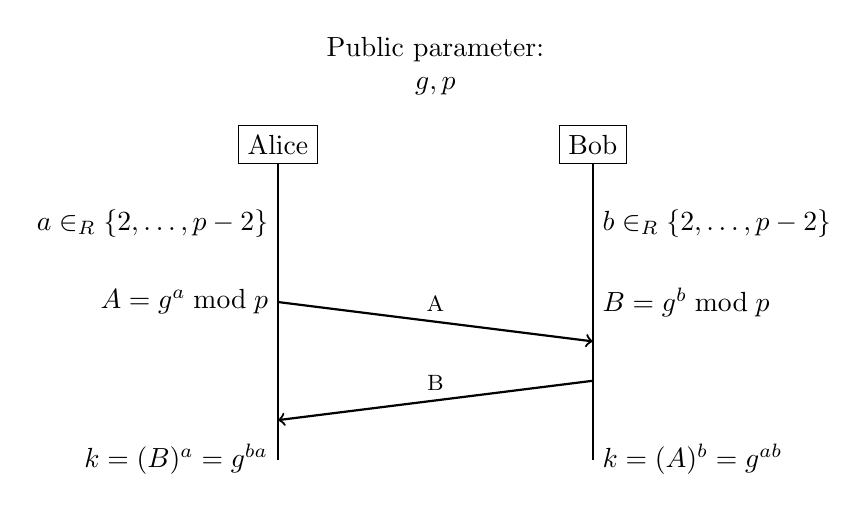
\begin{tikzpicture}
  % Public parameter:
  \node[draw=none,fill=none,align=center] (public) at (0,1) {Public parameter:\\$g, p$};
  
  % Alice
  \node[draw] (Alice) at (-2,0) {Alice}; 
  \draw[thick] (Alice) -- ++(0, -4);
    
  % Calculations of Alice
  \node[draw=none,fill=none,anchor=east] (asecret) at ($(Alice) + (0,-1)$) {$a \in_{R} \{2,\dots,p-2\}$};
  \node[draw=none,fill=none,anchor=east] (Apublic) at ($(Alice) + (0,-2)$) {$A = g^{a} \bmod{p}$};
  \node[draw=none,fill=none,anchor=east] (akey) at ($(Alice) + (0,-4)$) {$k = (B)^{a} = g^{ba}$};
    
  % Bob
  \node[draw] (Bob) at (2,0) {Bob}; 
  \draw[thick] (Bob) -- ++(0, -4);
   
  % Calculations of Bob
  \node[draw=none,fill=none,anchor=west] (bsecret) at ($(Bob) + (0,-1)$) {$b \in_{R} \{2,\dots,p-2\}$};
  \node[draw=none,fill=none,anchor=west] (Bpublic) at ($(Bob) + (0,-2)$) {$B = g^{b} \bmod{p}$};
  \node[draw=none,fill=none,anchor=west] (bkey) at ($(Bob) + (0,-4)$) {$k = (A)^{b} = g^{ab}$};
   
  % Messages
  \draw[->,thick] ($(Alice)+(0,-2)$) -- ($(Bob)+(0,-2.5)$) node [pos=0.5,above,font=\footnotesize] {A};
  \draw[->,thick] ($(Bob)+(0,-3)$) -- ($(Alice)+(0,-3.5)$) node [pos=0.5,above,font=\footnotesize] {B};
    
\end{tikzpicture}
\end{center}
\caption{Alice and Bob's execution of Diffie-Hellman key exchange.}
\label{fig:diffiehellman}
\end{figure}

\subsection{Interactive Identification Schemes}

Imagine Alice wishes to confirm the identity of Bob. The idea behind interactive identification protocols is to offer Bob some way of proving to Alice (or anyone) that he has knowledge of some secret which \textbf{only} Bob could possess. The goal, of course, being to accomplish this without openly revealing the secret, so that it can continue to be used as an identifier for Bob. 

An identification scheme (or otherwise ``proof of identity") $\Pi_{id}$ is composed of by the tuple of polynomial-time algorithms (\textbf{KeyGen}, \textbf{Prove}, \textbf{Verify}). $\Pi_{id}$ is an interactive protocol, wherein the \emph{prover} (Bob, for example) 
executes \textbf{Prove} and the \emph{verifier} (Alice) executes \textbf{Verify}.

Execution of $\Pi_{id}$ between Alice and Bob involves the following:
\begin{enumerate}[label=(\roman*)]
\item Bob runs $\textbf{KeyGen}(1^\lambda)$: A probabilistic algorithm with input $1^\lambda$ and output $(sk,pk)$. 
\item Bob sends to Alice his public key $pk$ and a probabilistically generated initial commitment $com$. Alice will respond with a \emph{challenge} value $ch$.
\item Bob runs $\textbf{Prove}(sk, com, ch)$: A deterministic algorithm with input $sk$ (Bob's secret key) and $ch$ (challenge) and output $resp$.
\item Alice runs $\textbf{Verify}(pk, com, ch, resp)$: A deterministic algorithm with input $pk$ (Bob's public key), $com$, $ch$, and $resp$ and output $b \in {0,1}$. Bob has successfully proven his identity to Alice if $b = 1$.
\end{enumerate}

If Alice accepts Bob's response, and $b = 1$, then we refer to the tuple $(com,ch,resp)$ as an \emph{accepting transcript}. In terms of security, it is common to show that an identification scheme is secure against \emph{impersonation} under a \emph{passive attack}. Proving such security implies that an adversary who eavesdrops on arbitrarily many executions of $\Pi_{id}$ between a verifier $\mathcal{V}$ and a prover $\mathcal{P}$ cannot successfully impersonate $\mathcal{V}$.

There exist variations upon this type of primitive wherein Alice is not required to send Bob a specific challenge value. These are known as \emph{non-interactive} identification schemes, or non-interactive proofs of identity (NIPoI). These non-interactive approaches to solving the problem of identity and \emph{authentication} further bridge the gap between identification protocols and signature schemes. 

\subsection{Signature Schemes}

We define a signature scheme as the tuple of algorithms $\Pi_{sig}$ = (\textbf{KeyGen}, \textbf{Sign}, \textbf{Verify}). Some execution of $\Pi_{sig}$ between Alice and Bob for a particular message $m$ sent from Bob to Alice involves the following...
\noindent
First, before any message is to be signed, the Bob must run the following:
\begin{itemize}
\item Bob runs $\textbf{KeyGen}(1^\lambda)$: A probabilistic algorithm with input $1^\lambda$ and output $(sk,pk)$.
\end{itemize}
Then, for every message $m$ Bob wishes to authenticate and send to Alice: 
\begin{enumerate}[label=(\roman*)]
\item Bob sends his public key $pk$ to Alice over an authenticated channel if he has not yet done so.
\item Bob runs $\textbf{Sign}(sk, m)$: A probabilistic algorithm with input $sk$ (Bob's secret key) and $m$ (the message Bob wishes to authorize) and output $\sigma$, known as a \emph{signature}.
\item Bob sends $m$ and $\sigma$ to Alice.
\item Alice runs $\textbf{Verify}(pk, m, \sigma)$: A deterministic algorithm with input $pk$ (Bob's public key), $m$, and $\sigma$ and output $b \in \{0,1\}$. Alice has confidence in the \emph{integrity} and origin \emph{authenticity} of $m$ if $b = 1$.
\end{enumerate}

As previously alluded to, it is worth noting that signature protocols and identification schemes are closely related. In essence, they are rather similar; but with two main differences. The first is rather comparable to the aforementioned difference between interactive identification schemes and non-interactive identification schemes. The second arises as a result of aiming to authenticate Bob on any particular message $m$. To achieve this, the signature scheme needs to be run every time Bob wishes to send a message to Alice. The details of this comparison are intentionally left vague, as it will from a topic of close inspection in section 2.4.

The strongest security goal for a signature scheme $\Pi_{sig}$ is expressed as \emph{existential unforgeability} under an \emph{adaptive chosen-message attack}. If this goal is provably satisfied, an adversary with the ability to sign arbitrary messages will not be able to forge any conceivable and valid signature.

\section{Algebraic Geometry \& Isogenies}
\emph{Groups \& Varieties}. A \textbf{group} is a 2-tuple composed of a set of elements and a corresponding group operation (also referred to as the group \emph{law}). Given some group defined by the set $G$ and the operation $\cdot$ (written as $(G,\cdot)$) it is typical to refer to the group simply as $G$. If $\cdot$ is equivalent to some rational mapping\footnote{A rational map is a mapping between two groups which is defined by a polynomial function with rational coefficients.} $f_G: G \rightarrow G$, then the group $(G,\cdot)$ is said to form an \textbf{algebraic variety}. A group which is also an algebraic variety is referred to as an \textbf{algebraic group}.

$G$ is said to be an \emph{abelian} group if, in addition to the four traditional group axioms (closure, associativity, existence of an identity, existence of an inverse), $G$ satisfies the condition of commutitiviy. More formally, for some group $G$ with group operation $\cdot$, we say $G$ is an abelian group iff $x \cdot y = y \cdot x$ $\forall x, y \in G$. An algebraic group which is also abelian is referred to as an \textbf{abelian variety}.

\begin{tcolorbox}
\begin{definition}[Abelian Variety]
\label{defn:abelianvariety}
for some algebraic group $G$ with operation $\cdot$, we say $G$ is an \underline{abelian variety} iff $x \cdot y = y \cdot x$ $\forall x, y \in G$. 
\end{definition}
\end{tcolorbox}

For some group $(G,\cdot)$, some $x,y \in G$, and some rational mapping $f_G: G \rightarrow G$, let the following sequence of implications denote the classification of $(G,\cdot)$:

$$
\text{group } \xRightarrow[]{x\cdot y = f_G(x,y)} \text{algebraic group } \xRightarrow[]{x\cdot y = y\cdot x} \text{abelian variety }
$$

\noindent
\emph{Morphisms}. Let us again take for example some group $(G,\cdot)$. Let's also define some set $S_{(G,\cdot)}$ which contains every tuple $(x,y,z)$ for group elements $x,y,z$ which satisfy $x\cdot y = z$.
$$
S_{(G,\cdot)} = \{x,y,z \in G | x\cdot y = z\}
$$
Take also for example a second group $(H,*)$ and some map $\phi: G \rightarrow H$. $\phi$ is said to be \emph{structure preserving} if the following implication holds:
$$
(x,y,z) \in S_{(G,\cdot)} \Rightarrow (\phi(x),\phi(y),\phi(z)) \in S_{(H,*)}
$$

A \textbf{morphism} is simply the most general notion of a structure preserving map. More specifically, in the domain of algebraic geometry, we will be dealing with the notion of a \textbf{group homomorphism}, defined as follows:
\begin{tcolorbox}
\begin{definition}[Group Homomorphism]
\label{defn:homomorphism}
For two groups $G$ and $H$ with respective group operations $\cdot$ and $*$, a \underline{group homomorphism} is a structure preserving map $h: G \rightarrow H$ such that $\forall u, v \in G$ the following holds:
$$h(u \cdot v) = h(u) * h(v)$$
\end{definition}
\end{tcolorbox}

From this simple definition, two more properties of homomorphisms are easily deducible. Namely, for some homomorphism $h: G \rightarrow H$, the following properties hold:
\begin{itemize}
\item $h$ maps the identity element of $G$ onto the identity element of $H$, and
\item $h(u^{-1}) = h(u)^{-1}, \forall u \in G$
\end{itemize}

Furthermore, an \emph{endomorphism} is a special type of morphism in which the domain and the codomain are the same groups. We denote the set of enomorphisms defineable over some group $G$ as $\text{End}(G)$.
The \emph{kernel} of a particular homomorphism $h: G \rightarrow H$  is the set of elements in $G$ that, when applied to $h$, map to the identity element of $H$. We write this set as $ker(h)$, and it is much analogous to the familiar concept from linear algebra, wherein the kernel denotes the set of elements mapped to the zero vector by some linear map.
\vspace{10mm}

\subsection{Fields \& Field Extensions}
\label{subsec:fields}

A \textbf{field} is a mathematical structure which, while being similar to a group, demands additional properties. Fields are defined by some set $F$ and two operations: \emph{addition} and \emph{multiplication}. In order for some tuple $(F,+,\cdot)$ to constitute a field, it must satisfy an assortment of axioms:\\

\emph{Addition axioms}:
\begin{itemize}
\item (closure) If $x \in F$ and $y \in F$, then $x + y \in F$.
\item $+$ is commutative.
\item $+$ is associative.
\item $F$ contains an element 0 such that $\forall x \in F$ we have $0 + x = x$.
\item $\forall x \in F$ there is a corresponding element $-x \in F$ such that $x + (-x) = 0$.
\end{itemize}

\emph{Multiplication axioms}:
\begin{itemize}
\item (closure) If $x \in F$ and $y \in F$, then $x \cdot y \in F$.
\item $\cdot$ is commutative.
\item $\cdot$ is associative.
\item $F$ contains an element $1 \neq 0$ such that $\forall x \in F$ we have $x \cdot 1 = x$.
\item $\forall x \neq 0 \in F$ there is a corresponding element $x^{-1} \in F$ such that $x \cdot (x^{-1}) = 1$.
\end{itemize}

Additionally, a field $(F,+,\cdot)$ must uphold the \emph{distributive law}, namely:
$$
 x \cdot (y + z) = x \cdot y + x \cdot y \text{ holds } \forall x,y,z \in F
$$

While these axioms are known to be satisfied by the sets $\mathbb{Q}$, $\mathbb{R}$, and $\mathbb{C}$ with typically defined $+$ and $\cdot$, our focus will be on a particular class of field known as a \emph{finite field}. Finite fields, as the name suggests, are fields in which the set $F$ contains finitely many elements - we refer to the number of elements in $F$ as the \emph{order} of the field.

Let us take some prime number $p$. We can construct a finite field by taking $F$ as the set of numbers $\{0, 1, ... p-1\}$ and defining $+$ and $\cdot$ as addition and multiplication \emph{modulo p}. Finite fields defined in this fashion are denoted as $\mathbb{F}_p$, and have order $p$.
\begin{center}
$\forall x,y \in \mathbb{F}_p$, $x + y = (x + b) \mod{p}$, and\\
$\forall x,y \in \mathbb{F}_p$, $x \cdot y = (x \cdot b) \mod{p}$\\
\end{center}

For any given field $K$ there exists a number $q$ such that, for every $x \in K$, adding $x$ to itself $q$ times results in the additive identity 0. This number is referred to as the \emph{characteristic} of $K$, for which we write char($K$). Finite fields are the only type of field for which $\text{char}(K) > 0$. Furthermore, if the field in question is finite and has prime order, then the order and the characteristic are equivalent.

A particular field $K'$ is called an \emph{extension field} of some other field $K$ if $K \subseteq K'$. The complex numbers $\mathbb{C}$, for example, are an extension field of $\mathbb{R}$. A given field $K$ is \emph{algebraically closed} if there exists a root for every non-constant polynomial defined over $K$. If $K$ itself is not algebraically closed, we denote the extension of $K$ that is by $\overline{K}$. 

An algebraic group $G_a$ is defined over a field $K$ if each element $e \in G_a$ is also an element of the field $K$, and the corresponding $f_{G_a}$ is defined over $K$. To show that a particular algebraic group $G_a$ is defined over some field $K$ we will henceforth denote the group/field pairing as $G_a(K)$. Naturally, in the case where our field is a finite field of order $p$, we write $G_a(\mathbb{F}_p)$.

These algebraic structures are all important for building up to the concept of an \emph{isogeny}. The lowest-level object we will be concerned with when discussing the forthcoming isogeny-based protocols will typically be elements of abelian varieties. The lowest-level structure in the SIDH C codebase is a finite field element.\\

\noindent
\emph{Montgomery Arithmetic}\label{snip:montgomery}. We will now briefly discuss a technique for efficiently performing modular arithmetic. This method is widely deployed in cryptosystems centered around finite fields, and is abundantly used in the \sidh library that we will shortly be examining.

In 1985, Peter Montgomery introduced a method for efficiently computing the modular multiplication of two elements $a$ and $b$. The technique begins with the construction of some constant $R$, whose value depends solely on the modulus $N$ and the underlying computer architecture.\footnote{The specifics of how $R$ is constructed are beyond the scope of this dissertation; if they feel so inclined, the reader should refer to \cite{mont}}

With the retrieval of $R$, $aR \mod{N}$ and $bR \mod{N}$ are constructed and referred to as the Montgomery \emph{representation} of $a$ and $b$ respectively. Montgomery multiplication outlines an algorithm for computing $abR \mod{N}$ (the Montgomery product of $a$ and $b$), from which $ab \mod{N}$ can be recovered through conversion back to standard representation. Once in Montgomery representation, other arithmetic can be performed (including field element inversions) in order to leverage the performance improvement offered by Montgomery modular multiplication -- converting back to regular representation when necessary.

Applying Montgomery multiplication has the added benefit of decreasing the amount of field element inversions that need to be computed. Because of this, the technique is particularly relevant to this dissertation. We continue this discussion in section \ref{sec:pbinvimplementation}.

\subsection{Elliptic Curves}

An elliptic curve is an algebraic curve defined over some field $K$, the most general representation of which is given by
$$
y^2 + a_{1}xy + a_{3}y = x^3 + a_{2}x^2 + a_{4}x + a_6.
$$
This representation encapsulates elliptic curves defined over any field. If, however, we are dicussing curves defined specifically over a field $K$ such that $\text{char}(K) > 3$ (see \cite{silverman}), then the more compact form $y^2 = x^3 + ax + b$ can be applied (see Figure \ref{fig:groupop} for a geometric visualization). In this dissertation we will default to this second representation, as the schemes with which we are concerned will always be defined over $\mathbb{F}_p$ for some large prime $p$.

We can define a group structure over the points of a given elliptic curve (or any other smooth cubic curve). If we wish to define a group in accordance to a particular curve, we do so with the following notation:
$$
E: y^2 = x^3 + ax + b
$$
Wherein $E$ denotes the group in question, the elements of which are all the points (solutions) of the curve. Throughout much of this section, the words \emph{point} and \emph{element} can be used interchangeably.\\

\noindent
\emph{The Group Law}. The group operation we define for $E$, denoted $+$, is better understood geometrically than algebraically. Consider the following.

Given two elements $P$ and $Q$ of some arbitrary elliptic curve group $E$, we define $+$ geometrically as follows: drawing the line $L$ through points $P$ and $Q$, we follow $L$ to its third intersection on the curve (which is guaranteed to exist), which we will denote as $R = (x_R, y_R)$. We then set $P + Q = -R$, where $-R$ is the reflection of $R$ over the x-axis: $(x_R, -y_R)$. This descriptive definition of $+$ is suitable for all situations \emph{except} for when $L$ is tangent to $E$ or when $L$ is parallel to the y-axis. These cases will be covered in a short moment. See Figure \ref{fig:groupop} for an illustrated representation of this process.

\begin{figure}[!h]
\begin{tikzpicture}[scale=.75]
	\begin{scope}[xshift=5cm]
		%\draw[very thin,color=gray] (-3.9,-3.9) grid (3.9,3.9);  %background grid
		\draw[->] (-4.2,0) -- (4.2,0) node[right] {$x$};         %x-axis
		\draw[->] (0,-4.2) -- (0,4.2) node[above] {$y$};         %y-axis
		
		\plotcurve{-2}{2}
		
		\draw[fill] (-1.73,0.531) circle (0.1) node[right] {$P$};
		\draw[fill] (0.28,1.209) circle (0.1) node[right] {$Q$};
	\end{scope}
	
	\begin{scope}[xshift=17cm]
		%\draw[very thin,color=gray] (-3.9,-3.9) grid (3.9,3.9);  %background grid
		\draw[->] (-4.2,0) -- (4.2,0) node[right] {$x$};         %x-axis
		\draw[->] (0,-4.2) -- (0,4.2) node[above] {$y$};         %y-axis
		
		\plotcurve{-2}{2}
		
		\draw [] (-1.73,0.531) -- (1.564,1.642);
		\draw [dashed] (1.564,1.642) -- (1.564,-1.642);
		
		\draw[fill] (-1.73,0.531) circle (0.1) node[right] {$P$};
		\draw[fill] (0.28,1.209) circle (0.1) node[right] {$Q$};
		\draw[fill] (1.564,1.642) circle (0.1) node[right] {$R$};
		\draw[fill] (1.564,-1.642) circle (0.1) node[right] {$R' = P+Q$};
  \end{scope}
\end{tikzpicture}
\caption{$+$ acting over points $P$ and $Q$ of $y^2 = x^3 - 2x + 2$.}
\label{fig:groupop}
\end{figure}

The group operation $+$ is referred to as \emph{pointwise addition}. In order for $(E,+)$ to properly form a group under pointwise addition, it must satisfy the four group axioms:
\begin{itemize}
\item \emph{Closure}: Because elliptic curves are polynomials of degree of 3, we know any given line passing through two points $P$ and $Q$ of $E$ will pass through a third point $R$. The exceptions here are twofold. First, when $P = Q$ and thus our line is tangent to $E$, and second, when $Q = -P$ and our line is parallel with the y-axis. We resolve the first case nicely by defining $P + P$ by means of taking $L$ to be the line tangent to $E$ at point $P$. In the second case, $P + (-P)$, by group axiom, should yield the identity element of the group. We will define this element and resolve this issue below.  
\item \emph{Identity}: The identity element of elliptic curve groups, denoted as $\mathcal{O}$, is a specially defined point satisfying $P + \mathcal{O} = \mathcal{O} + P = P$, $\forall P \in E$. Because of the inclusion of this special element, we have that $\#(E(K))$ is equal to $1$ $+$ the number geometric points on $E$ defined over $K$. This of course is only a noteworthy claim when $K$ is a finite field (otherwise there are already infinitely many elements in $E$).
\item \emph{Associativity}: For all points $P$, $Q$, and $R$ in $E$, it must be the case ($(P + Q) + R = P + (Q + R)$) holds. It is rather easy to see visually why this is true for geometrically defined points in $E$ (see Figure \ref{fig:axioms}). Additionally, we can trivially show that this holds when any combination of $P$, $Q$, and $R$ are $\mathcal{O}$ by applying the axiom of the identity.
\item \emph{Inverse}: Due to the x-symmetry of elliptic curves, every point $P = (x_P, y_P)$ of $E$ has an associated point $-P = (x_P, -y_P)$. If we apply $+$ to $P$ and $-P$, $L$ assumes the line parrallel to the y-axis at $x = x_P$. As discussed above, in this case there is no third intersection of $L$ on $E$. In light of this, $\mathcal{O}$ can be thought of as a point residing infinitely far in both the positive and negative directions of the y-axis. $\mathcal{O}$ is equivalently referred to as the \emph{point at infinity} (see Figure \ref{fig:axioms}).\footnote{One might suspect that the inclusion of this (apparently) non-algebraic element $\mathcal{O}$ suggests that $+$ is not a rational-map. The operator $+$ \emph{can} be shown to be a rational-mapping if we define our elliptic curve groups in three-dimensional projective space.}
\end{itemize}

\begin{figure}[!h]
\begin{tikzpicture}[scale=.55]
	\begin{scope}[xshift=0cm]
		%\draw[very thin,color=gray] (-3.9,-3.9) grid (3.9,3.9);  %background grid
		\draw[->] (-4.2,0) -- (4.2,0) node[right] {$x$};         %x-axis
		\draw[->] (0,-4.2) -- (0,4.2) node[above] {$y$};         %y-axis
		
		\draw[] (-1.65,0.677) -- (2.00,1.414); 
		\draw[dashed] (-0.309,0.948) -- (-0.309,-0.948);
		\draw[] (-1.400,-1.207) -- (1.765,-0.454); 
		\draw[dashed] (1.765,-0.454) -- (1.765,0.454);
		
		\plotcurve{-3}{0}
		
		\draw[fill] (-1.65,0.677) circle (0.1) node[left] {$P$};
		\draw[fill] (2.00,1.414) circle (0.1) node[right] {$Q$};
		\draw[fill] (-0.309,0.948) circle (0.1) node[right] {};
		\draw[fill] (-0.309,-0.948) circle (0.1) node[right] {};
		\draw[fill] (-1.400,-1.207) circle (0.1) node[below] {$R$};
		\draw[fill] (1.765,-0.454) circle (0.1) node[right] {};
		\draw[fill] (1.765,0.454) circle (0.1) node[right] {$(P + Q) + R$};
	\end{scope}
	\begin{scope}[xshift=10cm]
		%\draw[very thin,color=gray] (-3.9,-3.9) grid (3.9,3.9);  %background grid
		\draw[->] (-4.2,0) -- (4.2,0) node[right] {$x$};         %x-axis
		\draw[->] (0,-4.2) -- (0,4.2) node[above] {$y$};         %y-axis
		
		\draw[] (2.00,1.414) -- (-1.400,-1.207);
		\draw[dashed] (-0.006,-0.132) -- (-0.006,0.132);
		\draw[] (-1.65,0.677) -- (1.765,-0.454);
		\draw[dashed] (1.765,-0.454) -- (1.765,0.454);
		
		\plotcurve{-3}{0}
		
		\draw[fill] (-1.65,0.677) circle (0.1) node[left] {$P$};
		\draw[fill] (2.00,1.414) circle (0.1) node[right] {$Q$};
		\draw[fill] (-1.400,-1.207) circle (0.1) node[below] {$R$};
		\draw[fill] (-0.006,-0.132) circle (0.1) node[right] {};
		\draw[fill] (-0.006,0.132) circle (0.1) node[right] {};
		\draw[fill] (1.765,-0.454) circle (0.1) node[right] {};
		\draw[fill] (1.765,0.454) circle (0.1) node[right] {$P + (Q + R)$};
	\end{scope}
	\begin{scope}[xshift=20cm]
		%\draw[very thin,color=gray] (-3.9,-3.9) grid (3.9,3.9);  %background grid
		\draw[->] (-4.2,0) -- (4.2,0) node[right] {$x$};         %x-axis
		\draw[->] (0,-4.2) -- (0,4.2) node[above] {$y$};         %y-axis
		
		\plotcurve{1}{1}
		
		\draw[dashed] (0.73,-4.492) -- (0.73,4.492);
		
		\draw[fill] (0.73,1.492) circle (0.1) node[right] {$P$};
		\draw[fill] (0.73,-1.492) circle (0.1) node[right] {$-P$};
  \end{scope}
\end{tikzpicture}
\caption{associativity illustrated on $y^2 = x^3 - 3x$ (left \& center) and $P + (-P) = \mathcal{O}$ illustrated for $y^2 = x^3 + x + 1$ (right).}
\label{fig:axioms}
\end{figure}

Of course, there are relatively simple formulas for algebraically defining point-wise addition and inverse computation. We have opted to describe these operations geometrically simply for ease of communication.

Additionally, we shorthand $\overbrace{P + P + ... + P}^{n}$ as $nP$, analogous to scalar multiplication.\\

Consequently, because groups defined over elliptic curves in this fashion are commutitive, they also constitute abelian varieties.

When referring to curves as abelian varieties defined over a field, we will write them as $E_{\alpha}(K)$, for some curve $E_{\alpha}$ and some field $K$. If we are only concerned with the geometric properties of the curve, or curves as distinct elements of some group structure, it will suffice to write $E_{\alpha}$. Moving forward from here, we will assume all general curves discussed are capable of definition over some finite field $\mathbb{F}_p$.\\

The $r$-\emph{torsion group} of $E$ is the set of all points $P \in E(\overline{\mathbb{F}}_q)$ such that $rP = \mathcal{O}$. We denote the $r$-torsion group of some curve as $E[r]$.\\

\noindent
\emph{Supersingular Curves}. An elliptic curve can be either \emph{ordinary} or \emph{supersingular}. There are several equivalent ways of defining supersingular curves (and thus the distinction between them and ordinary curves) in a general setting, but each of these goes well beyond our scope. In the context of curves defined over finite fiels, however, the following succinct definition holds:
\begin{tcolorbox}
\begin{definition}[Supersingular Curve]
\label{defn:supersingular}
Let $E$ be an elliptic curve defined over the finite field $\mathbb{F}_{p}$. $E$ is said to be \underline{supersingular} if $\#(E(\mathbb{F}_{p})) = p+1$.\footnote{Readers are welcomed to investigate \cite{pairings} for further details.}
\end{definition}
\end{tcolorbox}

For the remainder of this paper, unless otherwise noted, all elliptic curves in discussion will supersingular.\\ 

\noindent
\emph{Projective Space}\label{snip:projspace}. While elliptic curves are naturally defined in two-dimensional affine space, there are many benefits to expressing them through three-dimension projective coordinates. First and foremost, expressing curves in projective space allows us to reason geometrically about $\mathcal{O}$. This is done by defining a curve $E$ such that it resides in some two-dimension subspace of 3-space, the point $\mathcal{O}$ then resides at some point in 3-space outside of the residing plane of $E$. 

Representing a curve in 3-space requires some substitution of $x$ and $y$ coordinates, a typical forma for achieving this is the following:

$$
x = X/Z\quad
y = Y/Z\quad
Z = 1
$$

Such a representation of elliptic curve points offers more computationally efficient arithmetic over points. This is conceptually similar to the previously mentioned Montgomery arithmetic regarding finite field elements. Other substitutions offer different computational advantages, but the implementations we will discuss make use of this typical approach.

\subsection{Isogenies \& Their Properties}

\begin{tcolorbox}
\begin{definition}[Isogeny]
\label{defn:isogeny}
Let $G$ and $H$ be algebraic groups. An \underline{isogeny} is a morphism $h: G \rightarrow H$ possessing a finite kernel.
\end{definition}
\end{tcolorbox}

In the case of the above definition where $G$ and $H$ are abelian varieties (such as elliptic curves,) the isogeny $h$ is homomorphic between $G$ and $H$. Because of this, isogenies over elliptic curves (and other abelian varieties) inherit certain characteristics.\\
For an isogeny $h: E_{1} \rightarrow E_{2}$ defined over elliptic curves $E_1$ and $E_2$, the following holds:
\begin{itemize}
\item $h(\mathcal{O}) = \mathcal{O}$, and
\item $h(u^{-1}) = h(u)^{-1}, \forall u \in G$
\end{itemize}

If there exists some isogeny $\phi$ between curves $E_1$ and $E_2$ then $E_1$ and $E_2$ are said to be \emph{isogenous}. All supersingular curves are isogenous only to other supersingular curves. The equivalent statement holds for ordinary curves. With this in mind, we can concieve a sort of graph structure connecting all isogenous curves, these graphs pertaining to either the supersingular or ordinary variety of curves. 

We write $\text{End}(E)$ to denote the ring formed by all the isogenies acting over $E$ which are also endomorphisms. Note that $m$-repeated pointwise addition of a point with itself can equivalently be modelled by an endomorphism, we denote the application of such an endomorphism to a point $P$ as $[m]P$, such that $[m]: E \rightarrow E$ and $[m]P = mP$.

An important facet of isogenies is that they can be uniquely identified by their kernel. If $S$ is the group of points denoting the kernel of some isogeny $\phi$ with domain $E$, we write $\phi: E \rightarrow E/S$. Because the subgroup $S$ sufficiently identifies $\phi$, any given generator of $S$ equivalently identifies $\phi$. Therefore, if $R$ generates the subgroup $S$ we can write $\phi: E \rightarrow E/\langle R \rangle$. Moreover, we will have a specific interest in isogenies with kernels defined by some \emph{torsion subgroup}. 

\section{Supersingular Isogeny Diffie-Hellman}

This section will aim to accomplish two things. First, we will briefly explain the isogeny-level \& key-exchange-level procedures of the SIDH protocol. Second, we will illuminate how these procedures map onto Microsoft Research's C implementation of SIDH. In this regard, this section can be considered an attempt to meld two domains of SIDH functions \& procedures, in hopes of easing the navigation from the SIDH protocol to Microsoft's C implementation, and vice versa.

The original work of De Feo, Jao, and Plut outlines three different isogeny-based cryptographic primitives: Diffie-Hellman-esque key exchange, public key encryption, and the aforementioned zero-knowledge proof of identity. Because all three of these protocols require the same initialization and public parameters, we will begin by covering these parameters in detail. Immediately after, we will analyze the key exchange at a relatively high level. Our goal of this section is to explain in detail the algorithmic and cryptographic aspects of the ZKPoI scheme, as this forms the conceptual basis for the signature scheme we will be investigating. We begin with the key exchange protocol because its sub-routines are integral to the Yoo et al. signature implementation.

For the discussion that follows, we will assume every instance of an SIDH protocol occurs between two parties, \textcolor{blue}{A} and \textcolor{red}{B} (eg. \textcolor{blue}{Alice} \& \textcolor{red}{Bob},) for which we will colorize information particular to \textcolor{blue}{A} in \textcolor{blue}{blue} and \textcolor{red}{B} in \textcolor{red}{red}. This will include private keys \& public keys as well as the variables and constants used in their generation.\\

\noindent
\emph{Public Parameters}. As the name suggests, SIDH protocols work over supersingular curves (with no singular points). Let $\mathbb{F}_q = \mathbb{F}_{p^2}$ be the finite field over which our curves are defined, $\mathbb{F}_{p^2}$ denoting the quadratic extension field of $\mathbb{F}_{p}$.  $p$ is a prime defined as follows:
$$
p = \laea \lbeb \cdot f \pm 1
$$
Wherein $\la$ and $\lb$ are small primes (typically \textcolor{blue}{2} \& \textcolor{red}{3}, respectively) and $f$ is a cofactor ensuring the primality of $p$. We then define globally a supersingular curve $E_0$ defined over $\mathbb{F}_q$ with cardinality $(\laea \lbeb f)^2$. Consequently, the torsion group $E_0[\laea]$ is $\mathbb{F}_q$-rational and has $\la^{\ea - 1} (\la + 1)$ cyclic subgroups of order $\laea$, with the analogous statement being true for $E_0[\lbeb]$. Additionally, we include in the public parameters the bases $\agens$ and $\bgens$, generating $E[\laea]$ and $E[\lbeb]$ respectively. 

This brings our set of global parameters, G, to the following:\\
$$
G = \{p,E_0,\la,\lb,\ea,\eb,\agens,\bgens\}
$$



\subsection{SIDH Key Exchange}

This subsection will illustrate an SIDH key exchange run between party members \textcolor{blue}{Alice} and \textcolor{red}{Bob}. The general idea of the protocol can be surmised by the diagram below. In the scheme, \textbf{private keys} take the form of isogenies[ref] defined with domain $E$, and \textbf{public keys} are the associated co-domain curve of said isogenies.

\begin{center}
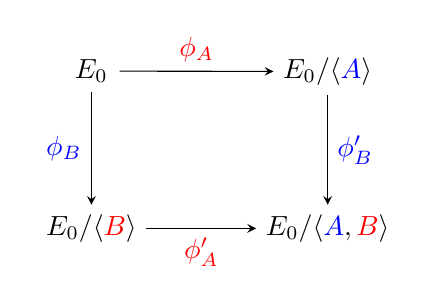
\begin{tikzpicture}
  \matrix (m) [matrix of math nodes,
               row sep=4em,
               column sep=4em,
               minimum width=2em] {
    E_0                     & E_0 / \langle \textcolor{blue}{A} \rangle    \\
    E_0 / \langle \textcolor{red}{B} \rangle & E_0 / \langle \textcolor{blue}{A}, \textcolor{red}{B} \rangle \\
  };
  \path[-stealth]
    (m-1-1) edge node [above] {$\pa$}  (m-1-2)
    (m-1-1) edge node [left]  {$\pb$}  (m-2-1)
    (m-2-1) edge node [below] {$\pap$} (m-2-2)
    (m-1-2) edge node [right] {$\pbp$} (m-2-2);
\end{tikzpicture}
\end{center}

The premise of the protocol is that both parties generate some random point (\textcolor{blue}{A} or \textcolor{red}{B} in the diagram,) which, according to theorem [ref], indicates some distinct isogeny $\phi_{\ba}: E_0 \rightarrow E/ \langle \ba \rangle$ (or equivalent for \rb). \textcolor{blue}{Alice} and \textcolor{red}{Bob} then exchange codomain curves and compute
\begin{center}
$\pa(E_0/\langle \rb \rangle)$\\
$\text{OR}$\\
$\pb(E_0/\langle \ba \rangle)$
\end{center}
To come to the shared secret agreement, the codomain curve of their composed isogenies, denoted $E_{\ba\rb}$. Below we've outlined the SIDH key exchange protocol $\Pi_{\text{SIDH}}$ = (\textbf{KeyGen}, \textbf{SecAgr}) in a descriptive (though not yet algorithmic) manner.\\

\noindent
\textbf{KeyGen($\lambda$)}: \textcolor{blue}{Alice} chooses two random numbers $\ma, \na \in \mathbb{Z}/\laea\mathbb{Z}$ such that $(\la \nmid \ma) \lor (\la \nmid \na)$. \textcolor{blue}{Alice} then computes the isogeny $\pa: E_0 \rightarrow E_{\ba}$ where $E_{\ba} = E_0 / \langle [\ma]\genpa, [\na]\genqa\rangle$ (equivalently, $ker(\pa) = \langle [\ma]\genpa, [\na]\genqa\rangle$). \bob undergoes the same procedure for random elements $\mb, \nb \in \mathbb{Z}/\lbeb\mathbb{Z}$.

\alice then applies her isogeny to the points which \bob will use in the creation of of his isogeny: $(\pa(\genpb),\pa(\genqb))$. \bob performs the analogous operation. This leaves us with the following private and public keys for \alice and \bob:

\begin{center}
$\ska = (\ma,\na)$\\
$\pka = (E_{\ba}, \pa(\genpb),\pa(\genqb))$\\
$\skb = (\mb,\nb)$\\
$\pkb = (E_{\rb}, \pb(\genpa),\pb(\genqa))$\\
\end{center}

\noindent
\textit{PK Exchange}: After \textcolor{blue}{Alice} and \textcolor{red}{Bob} successfully complete their key generation, they perform the following over an insecure channel:
\begin{itemize}
\item \alice sends \bob $(E_{\ba}, \{\pa(\genpb),\pa(\genqb)\})$
\item \bob sends \alice $(E_{\rb}, \{\pb(\genpa),\pb(\genqa)\})$
\end{itemize}

\noindent
\textbf{SecAgr($sk_{1}$,$pk_{2}$)}: After reception of \bob's tuple, \alice computes the isogeny $\phi'_A: E_{\rb} \rightarrow E_{\ba\rb}$ and \bob acts analogously. \alice and \bob then arrive at the equivalent image curve:
$$
E_{\ba\rb} = \phi'_{\ba}(\phi_{\rb}(E_0)) = \phi'_{\rb}(\phi_{\ba}(E_0)) = E_0/ \langle [\ma]\genpa + [\na]\genqa, [\mb]\genpb + [\nb]\genqb \rangle
$$
From which they can use the common j-invariant of as a shared secret $k$.

\begin{figure}[htb]
\centering
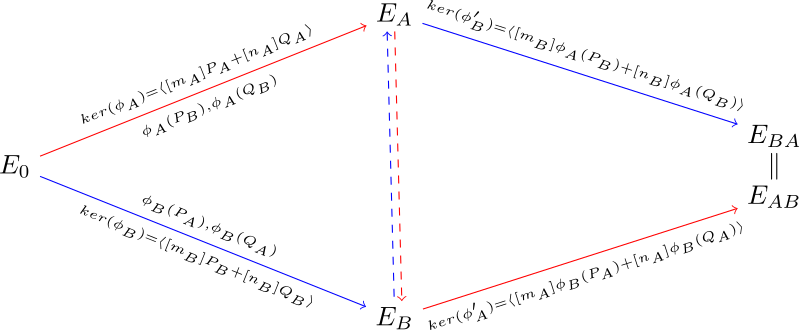
\includegraphics[scale=0.5]{keyexchange.png} % e.g. insert ./image for image.png in the working directory, adjust scale as necessary
\caption{SIDH key exchange between \textcolor{blue}{Alice} \& \textcolor{red}{Bob}}
\label{fig:kex} % insert suitable label, this is used to refer to a fig from within the text as shown above
\end{figure}

\subsection{Zero-Knowledge Proof of Identity}

Recall the earlier discussed notion of an identification scheme. A canonical identification scheme $\Pi_{\text{SID}} = (\textbf{KeyGen},\textbf{Prove},\textbf{Verify})$ can be derived somewhat analogously to the SIDH protocol, and is outlined in the original work of De Feo et al.

Say \bob has derived for himself the key pair $(\skb,\pkb)$ with $\skb = \{\mb,\nb\}$ and $\pkb = E_{\rb} = E_0/\langle [\mb]\genpb + [\nb]\genqb \rangle$ in relation to the public parameters $E_0$ and $\lbeb$. With $E_0$ and $E_{\rb}$ publicly known, $\Pi_{\text{ZKPoI}}$ revolves around \bob trying to prove to \alice that he knows the generator for $E_{\rb}$ without revealing it.

To achieve this, \bob internally mimicks an execution of the key exchange protocol $\Pi_{SIDH}$ with an arbitrary ``random" entity \randall.\\

\noindent
\textbf{KeyGen}: Key generation is performed exactly as in $\Pi_{\text{SIDH}}$, the only difference being that in $\Pi_{\text{ZKPoI}}$ only the prover (\bob, in our example,) needs to generate a keypair.\\

\noindent
\emph{Commitment}: \bob generates a random point $\cyr \in E_0[\laea]$ ($\cyr = [\mr]\genpa + [\nr]\genqa$) along with the corresponding isogenies necessary to compute the diagram below in full (if \alice were acting as the prover in $\Pi_{\text{ZKPoI}}$, then she would choose $\cyr \in E_0[\lbeb]$). \bob sends his commitment $com$ as $(com_1,com_2) = (E/\langle \cyr \rangle, E/\langle \rb, \cyr \rangle)$ to \alice.\\

\begin{center}
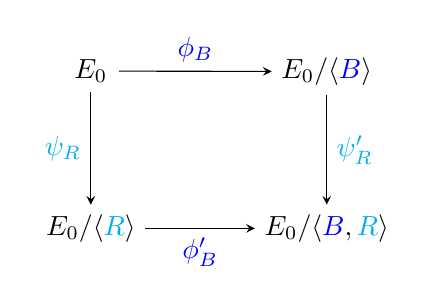
\begin{tikzpicture}
  \matrix (m) [matrix of math nodes,
               row sep=4em,
               column sep=4em,
               minimum width=2em] {
    E_0                     & E_0 / \langle \rb \rangle    \\
    E_0 / \langle \cyr \rangle & E_0 / \langle \rb, \cyr \rangle \\
  };
  \path[-stealth]
    (m-1-1) edge node [above] {$\pb$}  (m-1-2)
    (m-1-1) edge node [left]  {$\pr$}  (m-2-1)
    (m-2-1) edge node [below] {$\pbp$} (m-2-2)
    (m-1-2) edge node [right] {$\prp$} (m-2-2);
\end{tikzpicture}
\end{center}

\noindent
\emph{Response}: \alice chooses a bit $b$ at random and sends her challenge $ch = b$ to \bob.\\

\noindent
\textbf{Prove($sk$, $ch$)}: If \alice's challenge bit $ch = 0$ then \bob reveals the isogenies $\pr$ and $\prp$ (to do this, he can simply reveal the generators of the kernels of $\pr$ and $\prp$; $\cyr$ and $\pb(\cyr)$ respectively). This proves he knows the information necessary to form a shared secret with \randall \emph{if and only if} he happens to know the private key $\rb = \{[\mb]\genpb + [\nb]\genqb\}$. If $ch = 1$, \bob reveals the isogeny $\pbp$. This proves that \bob knows the information necessary to form a shared secret with \randall \emph{if and only if} he knows \randall's secret key $\cyr$.\\

\begin{center}
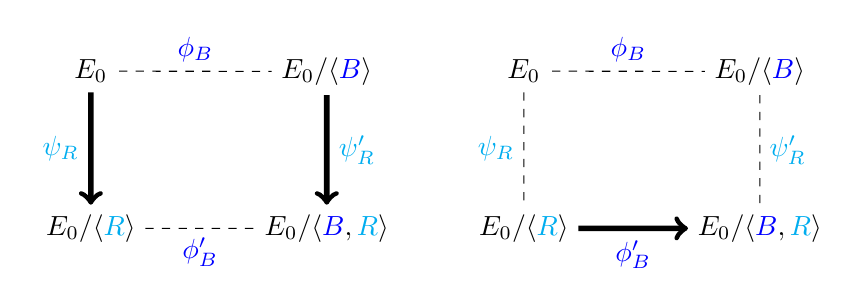
\begin{tikzpicture}[scale=.55]
	\begin{scope}[xshift=0cm]
		\matrix (m) [matrix of math nodes,
               row sep=4em,
               column sep=4em,
               minimum width=2em] {
    E_0                     & E_0 / \langle \rb \rangle    \\
    E_0 / \langle \cyr \rangle & E_0 / \langle \rb, \cyr \rangle \\
		};
		\draw[dashed] (m-1-1) edge node [above] {$\pb$}  (m-1-2);
		\draw[->, line width=2.0] (m-1-1) edge node [left]  {$\pr$}  (m-2-1);
		\draw[dashed] (m-2-1) edge node [below] {$\pbp$} (m-2-2);
		\draw[->, line width=2.0] (m-1-2) edge node [right] {$\prp$} (m-2-2);
	\end{scope}
	\begin{scope}[xshift=10cm]
		\matrix (m) [matrix of math nodes,
               row sep=4em,
               column sep=4em,
               minimum width=2em] {
    E_0                     & E_0 / \langle \rb \rangle    \\
    E_0 / \langle \cyr \rangle & E_0 / \langle \rb, \cyr \rangle \\
		};
		\draw[dashed] (m-1-1) edge node [above] {$\pb$}  (m-1-2);
		\draw[dashed] (m-1-1) edge node [left]  {$\pr$}  (m-2-1);
		\draw[->, line width=2.0] (m-2-1) edge node [below] {$\pbp$} (m-2-2);
		\draw[dashed] (m-1-2) edge node [right] {$\prp$} (m-2-2);
	\end{scope}
\end{tikzpicture}
\end{center}

Note that \bob cannot at once reveal all of the information necessary to convince \alice that he knows $\rb$. If he reveals $\cyr$, $\pb(\cyr)$, and $\pbp$ all in one go, he incidentally reveals his secret key $\rb = [\mb]\genpb + [\nb]\genqb$. This is because \bob reveals $\pbp$ by revealing the generator of $ker(\pbp)$, namely:
$$
(\rb, \cyr) = [\mb]\genpb + [\nb]\genqb, [\mr]\genpa + [\nr]\genqa \rangle
$$

How $\Pi_{\text{ZKPoK}}$ handles this is by having \bob and \alice run \textbf{Prove()} and \textbf{Verify()} for $\lambda$ iterations, with a different $(com, ch, resp)$ transcript generated for every instance. This way, if \bob is able to provide a $resp$ that satisfies \alice's $ch$ for every iteration, she can be sufficiently confident that \bob has knowledge of $\rb$.\\

\noindent
\textbf{Verify($pk, com, ch$)}: Like the proving procedure, verification is a conditional function depending on the value of $b$:
\begin{itemize}
\item if $ch = 0$: return 1 \emph{if and only if} $\cyr$ and $\pb(\cyr)$ have order $\laea$ and generate the kernels of isogenies from $E_0 \rightarrow E_0/\langle \cyr \rangle$ and $E_0/\langle \rb \rangle \rightarrow E_0/\langle \rb, \cyr \rangle$ respectively.
\item if $ch = 1$: return 1 \emph{if and only if} $\pr(\rb)$ has order $\lbeb$ and generates the kernel of an isogeny over $E_0/\langle \cyr \rangle \rightarrow E_0/\langle \rb, \cyr \rangle$.
\end{itemize}

This scheme constitutes what is known in the literature as a \emph{zero knowledge} proof of identity. It is referred to as such because \alice, acting as the verifier, does not gain any information about \bob's secret key $sk$.

\section{Fiat-Shamir Construction}

The Fiat-Shamir construction (also frequently referred to as the Fiat-Shamir transform, or Fiat-Shamir hueristic,) is a high-level technique for transforming a canonical identification scheme into a secure  signature scheme.

The construction is rather simple. The idea is to first transform a given interactive identification protocol $\Pi_{\text{ID}}$ into a \emph{non-interactive} identification protocol. To achieve this, instead of allowing input from the verifier $\mathcal{V}$, we have our prover $\mathcal{P}$ generate the challenge $ch$ by itself. In order for the verifier to be able to check that $ch$ was generated honestly, we define $ch = H(com)$, where $H$ is some secure hash function. If we model $H$ as a \emph{random oracle}[ref], $H(com)$ is truly random; from this it can be shown that it is just as difficult for an impersonator of $\mathcal{P}$ to find an accepting transcript $(com, H(com), resp)$ as it would be for them to successfully impersonate $\mathcal{P}$ in $\Pi_{\text{ID}}$.

Now that we've paired $\Pi_{\text{ID}}$ with $H$ to achieve a non-interactive identification scheme $\Pi_{\text{NID}}$, we need only to factor in some message $m$ from $\mathcal{P}$ to have constructed a signature scheme $\Pi_{\text{ID}}'$. This can be achieved by including $m$ in our calculation of the challenge: $ch = H(com, m)$. Therefore, given theorem \ref{thm:fiatshamir}, if $(com, H(com), resp)$ is an accepting transcript of $\Pi_{\text{NID}}$, then $(com, H(com, m), resp)$ is a secure signature for the message $m$. Of course, because $H(com, m)$ can be constructed by any passively observing party, it is redundant to include; and so $(com,resp)$ constitutes a valid signature for $m$. A proof of theorem \ref{thm:fiatshamir} can be found in \cite{sigs}. The security of the Fiat-Shamir construct was first proven by Pointcheval \& Stern in \cite{fsproof}.

\begin{tcolorbox}
\begin{theorem}[Fiat-Shamir Security]
\label{thm:fiatshamir}
Let $\Pi_{\text{ID}} = (\textbf{KeyGen}, \textbf{Prove}, \textbf{Verify})$ be a canonical identification scheme that is secure against a passive attack. Then, if $H$ is modeled as a random oracle, the signature scheme $\Pi_{\text{ID}}'$ that results from applying the Fiat-Shamir transform to $\Pi_{\text{ID}}$ is \emph{classically} existentially unforgeable under an adaptive chosen-message attack.
\end{theorem}
\end{tcolorbox}

We will write $\textbf{FS}(\Pi)$ to denote the result of applying the Fiat-Shamir transformation to some identification protocol $\Pi$.

\subsection{Unruh's Post-Quantum Adaptation}

In 2014, Ambainis et al. showed that classical security proofs for ``proof of knowledge" protocols are insecure in the quantum setting. This is due to a technique used in the proof of FST's security whereby the random oracle is subject to ``rewinding": the proof simulates multiple runs of FST with different responses from the random oracle \cite{rewinding}.

Following this insight, Unruh proposed in 2015 a construction based off that of Fiat \& Shamir which he proved to be secure in both the classical and quantum random oracle models.

Because the focus of this dissertation is not the security (post-quantum or otherwise) of any particular protocol, our coverage in this section is left brief. 

\section{Isogeny Based Signatures}

Since publication of the SIDH suite, there have been several attempts at providing authentication schemes within the same framework. The post-quantum community had demonstrated undeniable signatures\cite{jvsig}, designated verifier signatures\cite{sunsig}, and undeniable blind signatures\cite{seshsig} all within the framework of isogeny based systems. It was not until the work of Yoo et al., however, that an isogeny based protocol for general authentication was shown as demonstrably secure. This protocol, particularly its C implementation, is where we have decided to focus our efforts.

Now that we've seen the zero-knowledge proof of identity (ZKPoI) from \cite{djp} as well as Unruh's quantum-safe Fiat-Shamir adaption, we have presented all of the material necessary for an indepth analysis of the isogeny based signature scheme presented by Yoo et al. The signature protocol, which we'll denote as $\Sigma'$, is a near-trivial application of Unruh's construction to the SIDH ZKPoI. In this section we will refer to the SIDH ZKPoI as $\Sigma$.

$\Sigma'$ is defined in the traditional manner, by a tuple of algorithms for key generation, signing, and verifying: $\Sigma' = (\textbf{KeyGen()}, \textbf{Sign()}, \textbf{Verify()})$. As could be predicted, \textbf{KeyGen()} in $\Sigma'$ is defined identically to the key generation found in SIDH key exchange. \textbf{Sign()} and \textbf{Verify()} are defined as equivalent to \textbf{Prove()} and \textbf{Verify()} $\in$ \textbf{FS($\Sigma$)}, respectively.

For our discussion of the signature scheme, we will make use of the naming conventions used in section 2.3. That is, we will discuss $\Sigma'$ as occuring between entities \bob and \alice, with \bob imitating the role of an arbitrary third party \randall during \textbf{Sign}.

The public parameters used in $\Sigma'$ are the same as outlined above for all of the protocols found in \cite{djp}. Namely, we have $p = \laea\lbeb \cdot f \pm 1$ where $\laea = 2$, $\lbeb = 3$, and $f$ is a cofacter such that $p$ is prime. We also set as parameter the curve $E$ such that $\#(E(F_{p^2})) = (\laea\lbeb)^2$. And again, we include the sets of points $(\genpa, \genqa)$ and $(\genpb, \genqb)$ generating $E[\laea]$ and $E[\lbeb]$ respectively. We have chosen $E$ over the previously used $E_0$ simply for ease of notation.

\subsection{Algorithmic Definitions}

It will be useful for us to outline in more detail the procedures of $\Sigma'$, at the very least to ease the transition into our discussion of the C implementation. In this subsection we will look at isogeny-level algorithmic definitions for \textbf{KeyGen()}, \textbf{Prove()}, and \textbf{Verify()}, and then look at how these procedures can be expressed in terms of the procedures of $\Pi_{\text{SIDH}}$.\\

\noindent
\textbf{KeyGen($\lambda$, $User$)}: As previously mentioned, key generation in $\Sigma'$ is identical to $\Sigma$:\textbf{KeyGen($\lambda$)}, which in turn is identical to $\Pi_{\text{SIDH}}$:\textbf{KeyGen($\lambda$)}. We've included a parameter $User$ equaling either $\alice$ or $\bob$ -- this denotes whether the user running the procedure uses \textcolor{blue}{blue} or \textcolor{red}{red} constants. We've also obfuscated the lower level details in regards to how points are generated and how isogenies can be constructed. We write $P_{User}$ and $Q_{User}$ for $\genpa$ \& $\genqa$ or $\genpb$ \& $\genqb$, depending on $User$.  The result is the following:

\begin{algorithm}
\caption{-- \textbf{KeyGen($\lambda$, $User$)}}\label{alg:keygensig}
\begin{algorithmic}[1]
\If{$User$ = $\alice$}
	\State Pick a random point $S$ of order $\laea$
\EndIf
\If{$User$ = $\bob$}
	\State Pick a random point $S$ of order $\lbeb$
\EndIf
\State Compute the isogeny $\phi: E \rightarrow E/\langle S \rangle$
\State $pk \gets (E/\langle S \rangle, \phi(P_{User}), \phi(Q_{User}))$
\State $sk \gets S$
\State \Return ($sk$, $pk$)
\end{algorithmic}
\end{algorithm}

\noindent
Transcribing this to the procedures of $\Pi_{\text{SIDH}}$ we arrive (quite trivially) at:\\

\begin{algorithm}
\caption{-- \textbf{KeyGen($\lambda$)}}\label{euclid}
\begin{algorithmic}[1]
\State ($sk$, $pk$) $\gets \Pi_{\text{SIDH}}$:\textbf{KeyGen($\lambda$)}
\State \Return ($sk$, $pk$)
\end{algorithmic}
\end{algorithm}

For \textbf{Sign($sk$, $m$)} and \textbf{Verify($pk$, $m$, $\sigma$)} we assume \bob to be the signer and \alice to be the verifier. Consequently, we will write the signers key pair ($sk$, $pk$) as ($\rb$, $\pb$). Algorithms for which the roles are reversed can be constructed simply by replacing \textcolor{red}{red} constants with their \textcolor{blue}{blue} correspondants, and vice-versa.\\  

\noindent
\textbf{Sign($sk$, $m$)}: The sign procedure, as a consequence of the Unruh construction, makes use of two random oracle functions \textbf{H} amd \textbf{G}. In the sign algorithm below, make note of how \bob computes both commitments and their corresponding responses for every iteration $i$ before he computes the challenge values (the bits of $J$). He then uses the $2\lambda$ bits of $J$ to decide which responses to include in $\sigma$.\\

\begin{algorithm}
\caption{-- \textbf{Sign($sk = \rb$, $m$)}}\label{euclid}
\begin{algorithmic}[1]
\For{\texttt{i = 1..2$\lambda$}}
	\State Pick a random point $\cyr$ of order $\laea$
	\State Compute the isogeny $\pr: E \rightarrow E/\langle \cyr \rangle$
	\State Compute either $\pbp : E/\langle \rb \rangle \rightarrow E/\langle \rb,\cyr \rangle$ or $\prp : E/\langle \cyr \rangle \rightarrow E/\langle \cyr,\rb \rangle$
	\State $(E_{1},E_{2}) \gets (E/\langle \cyr \rangle, E/\langle \cyr,\rb \rangle)$
	\State $com_{i} \gets (E_{1}, E_{2})$
	\State $ch_{i,0} \gets_{R} \{0,1\}$
	\State $(resp_{i,0}, resp_{i,1}) \gets ((\cyr,\pb(\cyr)), \pr(\rb))$
	\If{$\texttt{ch}_{i,0} = 1$}
		\State \textbf{Swap($resp_{i,0}$,$resp_{i,1}$)}
	\EndIf
	\State $h_{i,j} \gets$ \textbf{G($resp_{i,j}$)}
\EndFor

\State $J_{1} \parallel ... \parallel J_{2\lambda} \gets$ \textbf{H($\pb$, $m$, $(com_{i})_{i}$,$(ch_{i,j})_{i,j}$,$(h_{i,j})_{i,j}$)}

\State \Return $\sigma \gets ((com_{i})_{i}, (ch_{i,j})_{i,j}, (h_{i,j})_{i,j}, (resp_{i,J_{i}})_{i})$
\end{algorithmic}
\end{algorithm}

\noindent
If we write out \textbf{Sign()} using the $\Pi_{\text{SIDH}}$ API, we see that the only real computation is being performed by \textbf{KeyGen()} and \textbf{SecAgr()}, and our two random oracles \textbf{H()} and \textbf{G()}.  The rest of the algorithm is merely organizing the information we've generated into the transcript ($com$, $ch$, $resp$) and then finally into $\sigma$.

\begin{algorithm}
\caption{-- \textbf{Sign($sk = \rb$, $m$)} via $\Pi_{\text{SIDH}}$}\label{euclid}
\begin{algorithmic}[1]
\For{\texttt{i = 1..2$\lambda$}}
	\State $(\cyr,\pr) \gets \Pi_{\text{SIDH}}$:\textbf{KeyGen($\lambda$, $\alice$)}
	\State $\pbp: E/\langle \rb \rangle \rightarrow E/\langle \rb,\cyr \rangle \gets \Pi_{\text{SIDH}}$:\textbf{SecAgr($\rb$, $\pr$)}
	\State $(E_{1},E_{2}) \gets (E/\langle \cyr \rangle, E/\langle \rb,\cyr \rangle)$
	\State $com_{i} \gets (E_{1}, E_{2})$
	\State $ch_{i,0} \gets_{R} \{0,1\}$
	\State $(resp_{i,0}, resp_{i,1}) \gets ((\cyr,\pb(\cyr)), \pr(\rb))$
	\If{$\texttt{ch}_{i,0} = 1$}
		\State \textbf{Swap($resp_{i,0}$,$resp_{i,1}$)}
	\EndIf
	\State $h_{i,j} \gets$ \textbf{G($resp_{i,j}$)}
\EndFor

\State $J_{1} \parallel ... \parallel J_{2\lambda} \gets$ \textbf{H($\pb$, $m$, $(com_{i})_{i}$,$(ch_{i,j})_{i,j}$,$(h_{i,j})_{i,j}$)}

\State \Return $\sigma \gets ((com_{i})_{i}, (ch_{i,j})_{i,j}, (h_{i,j})_{i,j}, (resp_{i,J_{i}})_{i})$
\end{algorithmic}
\end{algorithm}


\noindent
\textbf{Verify($pk$, $m$, $\sigma$)}: \alice begins her execution of \textbf{Verify()} where \bob ended his execution of \textbf{Sign()}, with the computation of $J$. \alice then knows at each iteration what check to perform on \bob's response, based on a conditional branch. You will notice that \bob's secret key $\rb$ occurs in the negative path of this branch; this is not a security concern because it is actually the point $\pr(\rb)$ that is communicated in $\sigma$, from which $\rb$ cannot be recovered.\\

\begin{algorithm}[H]
\caption{-- \textbf{Verify($pk = \pb$, $m$, $\sigma$)}}\label{euclid}
\begin{algorithmic}[1]
\State $J_{1} \parallel ... \parallel J_{2\lambda} \gets$ \textbf{H($\pb$, $m$, $(com_{i})_{i}$,$(ch_{i,j})_{i,j}$,$(h_{i,j})_{i,j}$)}
\For{\texttt{i = 0..2$\lambda$}}
	\State \textbf{check} $h_{i,J_{i}} = G(resp_{i,J_{i}})$
	\If{$ch_{i,J_{i}} = 0$}
		\State Parse $(\cyr,\pb(\cyr)) \gets resp_{i,J_{i}}$
		\State \textbf{check} $(\cyr, \pb(\cyr))$ have order $\laea$
		\State \textbf{check} $\cyr$ generates the kernel of the isogeny $E \rightarrow E_{1}$
		\State \textbf{check} $\pb(\cyr)$ generates the kernel of the isogeny $E/\langle \rb \rangle \rightarrow E_{2}$
	\Else
		\State Parse $\pr(\rb) \gets resp_{i,J_{i}}$
		\State \textbf{check} $\pr(\rb)$ has order $\lbeb$
		\State \textbf{check} $\pr(\rb)$ generates the kernel of the isogeny $E_{1} \rightarrow E_{2}$
	\EndIf
\EndFor

\If{all checks succeed}
	\State \Return 1
\Else
	\State \Return 0
\EndIf
\end{algorithmic}
\end{algorithm}

\noindent
What we are checking for in the verification process is whether or not \bob and \randall performed an honest and valid key exchange. And so, if the challenge bit is 0, we can use SIDH key generation to determine that $\cyr$ and $\pr$ are a valid key pair and then run SIDH secret agreement with $\cyr$ and \bob's public key $\pb$ to confirm that it properly executes outputting an isogeny with kernel generated by $\pb(\cyr)$. If the challenge bit is 1, we can run an instance of SIDH secret agreement to verify that $\pr(\rb)$ generates the kernel of an isogeny with domain $E_{1}$ and co-domain $E_{2}$ (refer again to the diagrams outlining \textbf{Prove} of section 2.3.2).

These observations are formalized in Algorithm 6, where we rewrite $\Sigma'$:\textbf{Verify()} in terms of $\Pi_{\text{SIDH}}$ procedure calls. Note, in line 10 of Algorithm 6, the call $\Pi_{\text{SIDH}}$:\textbf{SecAgr($\pr(\rb)$, $\pr$)}. It should be noted that $\pr(\rb)$ is not the proper secret key input used by \bob in \textbf{Sign()}, but we will see in the section to follow how we can use $\pr(\rb)$ in the C implementation of \textbf{SecAgr} to perform our verification (without compromising \bob's secret key $\rb$).

\begin{algorithm}[H]
\caption{-- \textbf{Verify($pk = \pb$, $m$, $\sigma$)} via $\Pi_{\text{SIDH}}$}\label{euclid}
\begin{algorithmic}[1]
\State $J_{1} \parallel ... \parallel J_{2\lambda} \gets$ \textbf{H($\pb$, $m$, $(com_{i})_{i}$,$(ch_{i,j})_{i,j}$,$(h_{i,j})_{i,j}$)}
\For{\texttt{i = 0..2$\lambda$}}
	\State \textbf{check} $h_{i,J_{i}} = G(resp_{i,J_{i}})$
	\If{$ch_{i,J_{i}} = 0$}
		\State Parse $(\cyr,\pb(\cyr)) \gets resp_{i,J_{i}}$
		\State \textbf{check} $(\cyr, \pr)$ is a valid output of $\Pi_{\text{SIDH}}$:\textbf{KeyGen($\lambda$, $\alice$)}
		\State \textbf{check} that $\Pi_{\text{SIDH}}$:\textbf{SecAgr($\cyr$, $\pb$)} successfully outputs an isogeny with co-domain $E_{2}$
	\Else
		\State Parse $\pr(\rb) \gets resp_{i,J_{i}}$
		\State \textbf{check} that $\Pi_{\text{SIDH}}$:\textbf{SecAgr($\pr(\rb)$, $\pr$)} successfully outputs an isogeny with co-domain $E_{2}$
	\EndIf
\EndFor

\If{all checks succeed}
	\State \Return 1
\Else
	\State \Return 0
\EndIf
\end{algorithmic}
\end{algorithm}

\section{Implementations of Isogeny Based Cryptographic Protocols}

Having now introduced all of the background material necessary for understanding SIDH and the isogeny based signature scheme in detail, we will investigate the portions of the SIDH C library which are relevent to our contributions.

The SIDH C library, written by a research team at Microsoft Research, was released in 2016 alongside an article titled \emph{Efficient Algorithms for Supersingular Isogeny Diffie-Hellman} (see \cite{effalg}). The article in question details several adjustments to the algorithms and data-representations outlined in \cite{djp}, leading to improved performance and key-sizes. Their C implementation (which we will henceforth refer to as \sidh) is built on top of these improved algorithms and tailored to a specific set of parameters, all-in-all offering 128-bit quantum security and 192-bit classical security key exchange up to 2.9 times faster than any previous implementation. We will look at some of the details of \sidh below. 

Before proceeding, it may be advisable to briefly overview the section on notation (\ref{sub:notation}) if one has not already.

\subsection{Parameters \& Data Representation}

\noindent
\emph{Parameters}. \sidh operates over the underlying basefield $\mathbb{F}_{p}$ where $p = \laea\cdot\lbeb - 1$, with $\la = 2$, $\lb = 3$, $\ea = 372$, and $\eb = 239$, giving $p$ a bitlength of 751. Now, recall the Montgomery representation of a curve:
$$
By^2 = Cx^3 + Ax^2 + Cx
$$

\sidh uses the public parameter curve $E$ defined in Montgomery form with $A = 0$, $B = 1$, and $C = 1$. The point pairs ($\genpa,\genqa$) and ($\genpb, \genqb$), generating $E[\laea]$ and $E[\lbeb]$ respectively, are hard-coded as an array of bytes. This set of parameters (including related data such as the bitlength of certain constants) is referred to in the system as \code{SIDHp751}, and is stored in the struct \code{CurveIsogenyStaticData} which will be outlined below.\\

\noindent
\emph{Data Structures}. There are several custom-defined data structures that are integral to \sidh. Below, we will briefly cover the ones which are likely to arise in our discussion:\\

\emph{Field elements}
\begin{itemize}
	\item \code{felm\_t} -- buffer of bytes representing elements of $\mathbb{F}_{p}$.
	\item \code{f2elm\_t} -- pair of \code{felm\_t} representing elements of $\mathbb{F}_{p^2}$.
\end{itemize}

\emph{Elliptic curve points}
\begin{itemize}
	\item \code{point\_affine} -- an \code{f2elm\_t} \code{x} and an \code{f2elm\_t} \code{y} representing a point in affine space.
	\item \code{point\_proj} -- an \code{f2elm\_t} \code{X} and an \code{f2elm\_t} \code{Z} representing a point as projective XZ Montgomery coordinates.
	\item \code{point\_full\_proj} -- \code{f2elm\_t} elements \code{X}, \code{Y}, and \code{Z} representing a point in projective space.
	\item \code{point\_basefield\_affine} -- an \code{felm\_t} \code{x} and an \code{felm\_t} \code{y} representing a point in affine space over the base field.
	\item \code{point\_basefield\_proj} -- an \code{felm\_t} \code{X} and an \code{felm\_t} \code{Z} representing a point as projective XZ Montgomery coordinates over the base field.
\end{itemize}

\emph{Crypto structures}
\begin{itemize}
	\item \code{publickey\_t} -- three \code{f2elm\_t}s representing a public key.\\
	\code{publickey\_t[0]} = users private isogeny applied to the other parties generator $P_x$\\
	\code{publickey\_t[1]} = users private isogeny applied to the other parties generator $Q_x$\\
	\code{publickey\_t[2]} = users private isogeny applied $P_x - Q_x$
\end{itemize}

\emph{Curve structures}
\begin{itemize}
	\item \code{CurveIsogenyStruct} -- Structure containing all necessary public parameter data.
	\item \code{CurveIsogenyStaticData} -- The same as \code{CurveIsogenyStruct}, but with buffer sizes fixed for \code{SIDHp751}.
\end{itemize}

The reader may note that \code{publickey\_t} does not contain any information defining the users co-domain curve $E/\langle S \rangle$ (with $S$ as the users secret key). It just so happens that in $\Pi_{\text{SIDH}}$ key exchange, the curves $E/\langle \ba \rangle$ and $E/\langle \rb \rangle$ are simply intermediary steps (useful for conceptualizing the protocol) and not necessary for computing the shared secret $j(E_{\ba\rb})$.

\subsection{Design Decisions}

\noindent
\emph{Projective Space}. As is common in ECC, a vast majority of the procedures of \sidh operate over the \emph{projective space}(\ref{snip:projspace}) representation of elliptic curve points. This widely-deployed technique is used to avoid the substantial cost of field element inversions (computing $x^{-1}$ for some element $x \in \mathbb{F}_{p^2}$). This means the majority of our calculations are performed over \code{point\_proj} structures using \emph{montgomery arithmetic}(\ref{snip:montgomery}) and converted to \code{point\_affine} when necessary. This general design strategy is highly related to our first contribution, which will be elaborated upon in the sections to come.\\

\noindent
\emph{Secret Keys}. Recall the origin of an $\Pi_{\text{SIDH}}$ private key $(m, n)$: the goal is to randomly select a generator of the torsion group $E[\laea]$ (or $E[\lbeb]$ for \bob). It is noted in \cite{djp} that any generator of the required torsion group is sufficient. It is also noted that $m$, unless equal to the order of the torsion group, is invertible. Because of this, \alice, for example, can simple compute $R = \genpa + [m^{-1}n]\genqa$, thus enabling secret keys to be stored as a single $\mathbb{F}_{p^2}$ element (which is referred to as $m$). This technicality has been implemented in \sidh, which both saves on storage as well as offers a means for generating secret keys that is more efficient than the trivial scalar multiplication and point-wise addition approach to computing $[m]P + [n]Q$.\\

\noindent
\emph{Tailor-made Montgomery Multiplication}.

\subsection{Key Exchange \& Critical Functions}
\label{subsec:functions}

There are 3 central modules (C file) in \sidh, all dealing with different levels of abstraction in the $\Pi_{\text{SIDH}}$ protocol. Operating at the lowest abstraction level is the module \code{fpx.c}, wherein functions for manipulating $\mathbb{F}_{p}$ and $\mathbb{F}_{p^2}$ elements are defined. One level up from \code{fpx.c} we have \code{ec\_isogeny.c}, containing functions pertaining to elliptic curves and point arithmetic (such as \code{j\_inv(...)} for computing the j-invariant of a curve and \code{secret\_pt(...)} for computing a users secret point $S$ given their private key $m$). The final, highest abstraction-level module we will discuss is \code{kex.c}. \code{kex.c} contains the protocol-level functions for performing $\Pi_{\text{SIDH}}$, namely \code{KeyGeneration\_A(...)} and \code{KeyGeneration\_B(...)} for generating \alice and \bob's private and public keys, as well as \code{SecretAgreement\_A(...)} and \code{SecretAgreement\_B(...)} for completing the secret agreement from both sides of the key exchange. Figure \ref{fig:halfmap} illustrates the relationship between these modules and the abstraction levels of isogeny based key exchange.

\begin{figure}[!htb]
\centering
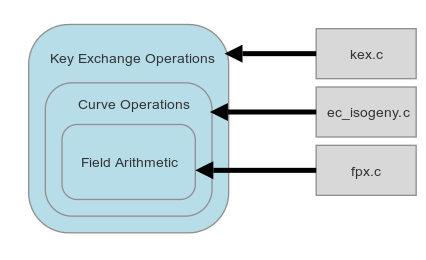
\includegraphics[scale=0.7]{halfmapwcurve.png} % e.g. insert ./image for image.png in the working directory, adjust scale as necessary
\caption{Relationship between $\Pi_{\text{SIDH}}$ \& \sidh modules}
\label{fig:halfmap} % insert suitable label, this is used to refer to a fig from within the text as shown above
\end{figure}

The estbalished notation for functions in \code{fpx.c} is to prepend function names with either \code{fp} or \code{fp2} to signify if it is defined for elements of $\mathbb{F}_{p}$ or $\mathbb{F}_{p^2}$. Additionally, it is common to append \code{\_mont} to the name of functions which are defined using Montgomery arithmetic. Functions in \code{fpx.c} are largely defined by byte and memory arithmetic, with the exception of slightly higher-level functions such as field element inversion (\code{fpinv751\_mont(...)}) which are defined in terms of other \code{fpx.c} functions. Furthermore, for efficiency, functions of \code{fpx.c} are defined as \code{\_\_inline} when applicable.

\code{ec\_isogeny.c} functions are defined almost exclusively in terms of \code{fpx.c} functions, with a few occurances of internal function calling. Functions in this module that are signifant to our our work are briefly surmised in figure \ref{fig:funcs}. The implementation specifics of most other \code{ec\_isogeny.c} functions are not critical to our work, and so have been excluded. The design and efficiency of these algorithms do, however, have a rich background and can be further read about in \cite{djp} and \cite{effalg}.

The key exchange procedures found in \code{kex.c} are composed entirely of calls to \code{fpx.c} and \code{ec\_isogeny.c} functions, modulo some basic branching logic.

\begin{center}
\code{fpx.c} functions\\
\begin{tabular}{|c|c|c|}
	\toprule
	Function & Input & Output\\
	\hline
	\code{to\_fp2mont} & \code{f2elm\_t a} & \code{f2elm\_t ma}\\
	Converts an $\mathbb{F}_{p^2}$  element & &\\
	to Montgomery representation & &\\
	\hline
	\code{from\_fp2mont} & \code{f2elm\_t ma} & \code{f2elm\_t a}\\
	Converts an $\mathbb{F}_{p^2}$ element & &\\
	from Montgomery representation  & &\\
	to regular form & &\\
	\hline
	\code{fp2inv751\_mont\_bingcd} & \code{f2elm\_t a} & \code{f2elm\_t a}$^{-1}$\\
	performs \emph{non-constant} & &\\
	time inversion of & &\\
	a $\mathbb{F}_{p^2}$ element & &\\
	\hline
	\code{fp2inv751\_mont} & \code{f2elm\_t a} & \code{f2elm\_t a}$^{-1}$\\
	performs \emph{constant} & &\\
	time inversion of & &\\
	a $\mathbb{F}_{p^2}$ element & &\\
	\bottomrule
\end{tabular}
\end{center}

\begin{center}
\code{ec\_isogeny.c} functions\\
\begin{tabular}{|c|c|c|}
	\toprule
	Function & Input & Output\\
	\hline
	\code{j\_inv} & \code{f2elm\_t A} & \code{f2elm\_t jinv}\\
	computes the j-invariant & \code{f2elm\_t C} &\\
	of a curve with represented & &\\
	in Montgomery form with \code{A} and \code{C} & &\\
	\hline
	\code{secret\_pt} & \code{point\_basefield P} & \code{point\_proj R}\\
	generates the secret & \code{digit\_t m} &\\
	point \code{R} from & \code{SIDHp751} &\\
	secret key \code{m} & \code{int AliceOrBob} &\\
	\hline
	\code{inv\_3\_way} & \code{f2elm\_t z1} & \code{f2elm\_t z1}$^{-1}$\\
	performs simultaneous inversion & \code{f2elm\_t z2} & \code{f2elm\_t z2}$^{-1}$\\
	of three elements & \code{f2elm\_t z3} & \code{f2elm\_t z3}$^{-1}$\\
	\hline
	\code{inv\_4\_way} & \code{f2elm\_t z1} & \code{f2elm\_t z1}$^{-1}$\\
	performs simultaneous inversion & \code{f2elm\_t z2} & \code{f2elm\_t z2}$^{-1}$\\
	of 4 elements & \code{f2elm\_t z3} & \code{f2elm\_t z3}$^{-1}$\\
	& \code{f2elm\_t z4} & \code{f2elm\_t z4}$^{-1}$\\
	\hline
	\code{generate\_2\_torsion\_basis} & \code{f2elm\_t A} & \code{point\_full\_proj R1}\\
	constructs a basis ($\{R1, R2\}$) & \code{SIDHp751} & \code{point\_full\_proj R2}\\
	generating $E[\laea]$ &  &\\
	\hline
	\code{generate\_3\_torsion\_basis} & \code{f2elm\_t A} & \code{point\_full\_proj R1}\\
	constructs a basis ($\{R1, R2\}$) & \code{SIDHp751} & \code{point\_full\_proj R2}\\
	generating $E[\lbeb]$ & &\\
	\bottomrule
\end{tabular}
\end{center}

\begin{center}
\code{kex.c} functions\\
\begin{tabular}{|c|c|c|}
	\toprule
	Function & Input & Output\\
	\hline
	\code{KeyGeneration\_A} & \code{unsigned char* privateKeyA} & \code{unsigned char* privateKeyA} \\
	performs key generation & \code{bool generateRandom} & \code{unsigned char* publicKeyA} \\
	for \alice & &\\
	\hline
	\code{KeyGeneration\_B} & & \code{unsigned char* privateKeyB}\\
	performs key generation & & \code{unsigned char* publicKeyB}\\
	for \bob & &\\
	\hline
	\code{SecretAgreement\_A} & \code{unsigned char* privateKeyA} & \code{unsigned char* sharedSecretA}\\
	computes the shared secret & \code{unsigned char* publicKeyB} & \code{point\_proj kerngen}\\
	from \alice's perspective & \code{point\_proj kerngen} &\\
	\hline
	\code{SecretAgreement\_B} & \code{unsigned char* privateKeyB} & \code{unsigned char* sharedSecretB}\\
	computes the shared secret & \code{unsigned char* publicKeyA} & \code{point\_proj kerngen}\\
	from \bob's perspective & \code{point\_proj kerngen} &\\
	\bottomrule
\end{tabular}
\end{center}

The reader may note that \code{privateKeyA} (in \code{KeyGeneration\_A}) and \code{kerngen} (in both secret agreements) appear as both inputs and outputs. This is no mistake. In \code{KeyGeneration\_A}, if \code{generateRandom = false} is passed as an input, then \code{privateKeyA} is expected to be set, and the corresponding public key is computed. In secret agreement, if \code{kerngen} is set to null then the algorithm proceeds normally. If it is set to a valid point, however, it can be used in place of a secret key input (which in such a case is expected to be null). Both of these details are critical to the design of signature functions as they are described below.

\subsection{Signature Layer}
\label{subsec:sigcode}

Yoo et al. provided, along with their publication of \cite{yoo}, an implementation of their signature scheme as a fork to \sidh. All of their functions are written specifically for an instance of $\Sigma'$ where the signer is assuming the \rb role (meaning that \randall assumes the \ba role), but their algorithms could be trivially modified to provide versions supporting a signer in the \ba role. Their contributions to the \sidh codebase come in the form of the functions listed below -- their relation to the rest of \sidh is illustrated in figure \ref{fig:fullmap}.

\begin{center}
\begin{tabular}{|c|c|c|c|}
	\toprule
	Function & Input & Output\\
	\midrule
	\code{isogeny\_keygen} & & \code{unsigned char* privateKeyB}\\
	generates the signers & & \code{unsigned char* publicKeyB}\\
	key pair & &\\
	\hline
	\code{isogeny\_sign} & \code{privateKey} & \code{Signature sig}\\
	produces a signature & \code{publicKey} &\\
	for a message & message $m$ &\\
	\hline
	\code{sign\_thread} & & \\
	performs a single iteration & &\\
	of the for-loop in \textbf{Sign} & &\\
	\hline
	\code{isogeny\_verify} & \code{Signature sig} & \code{true} or \code{false}\\
	checks the validity & &\\
	of a signature & &\\
	\hline
	\code{verify\_thread} & &\\
	performs a single iteration & &\\
	of the for-loop in \textbf{Verify} & &\\
	\bottomrule
\end{tabular}
\end{center}

To begin, \code{isogeny\_keygen} has a trivial definition; \code{KeyGeneration\_B} is called and populates the signer's public and private keys. \code{isogeny\_keygen} returns the success status of the call to \code{KeyGeneration\_B}.

In their original fork of \sidh, Yoo et al. included these functions in the file \code{kex\_tests.c}. This file was originally intended for testing the functions of \code{kex.c}, and so our fork of the library has placed the signature functions in a new file \code{SIDH\_signature.c}. We have also included a file \code{sig\_tests.c} for testing the contents and performance of \code{SIDH\_signature.c} functions. 

\begin{figure}[htp]
\centering
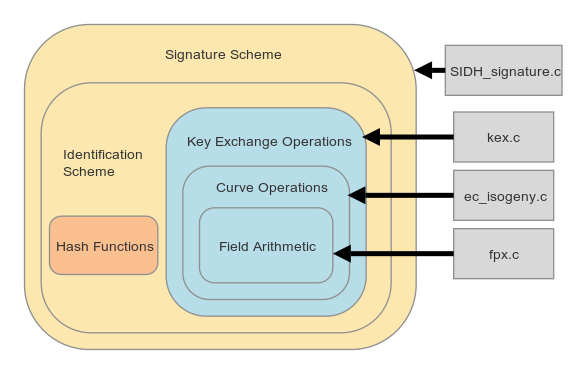
\includegraphics[scale=0.7]{fullmapwcurve.png} % e.g. insert ./image for image.png in the working directory, adjust scale as necessary
\caption{Relationship between SIDH based signatures \& Our fork of the SIDH C library}
\label{fig:fullmap} % insert suitable label, this is used to refer to a fig from within the text as shown above
\end{figure}

If we transcribe the procedures $\Sigma'$:\textbf{Sign} and $\Sigma'$:\textbf{Verify} as described in section 2.5 to the language of the \sidh API, we have in essense the following:\\

\begin{algorithm}
\caption{-- \code{Sign($sk_{\rb}$, $m$)}}\label{alg:signmath}
\begin{algorithmic}[1]
\For{\texttt{i = 1..2$\lambda$}}
	\State $(sk_{\cyr} = \cyr, pk_{\cyr}) \gets \code{KeyGeneration\_A(\code{NULL}, \code{true})}$
	\State $(E/\langle \rb,\cyr \rangle, \pr(\rb)) \gets \code{SecretAgreement\_B(}sk_{\rb}, pk_{\cyr}, \code{NULL})$
	\State $(E_{1},E_{2}) \gets (E/\langle \cyr \rangle, E/\langle \rb,\cyr \rangle)$
	\State $(\texttt{com}[i]_{0}, \texttt{com}[i]_{1}) \gets (E_{1}, E_{2})$
	\State $(\texttt{resp}[i]_{0}, \texttt{resp}[i]_{1}) \gets (\cyr, \pr(\rb))$
	\State $h[i] \gets$ \code{keccak(resp$[i]_0$)|keccak(resp$[i]_1$)}
\EndFor

\State $J_{1} \parallel ... \parallel J_{2\lambda} \gets$ \code{keccak(com, $m$, $h$)}

\State \Return $\sigma \gets ((\texttt{com}_{i})_{i}, (\texttt{ch}_{i,j})_{i,j}, (h_{i})_{i}, ((\texttt{resp})[J_{i}])$
\end{algorithmic}
\end{algorithm}

\begin{algorithm}[H]
\caption{-- \code{Verify($pk = \pb$, $m$, $\sigma$)}}\label{alg:verifmath}
\begin{algorithmic}[1]
\State $J_{1} \parallel ... \parallel J_{2\lambda} \gets$ \code{keccak(com, $m$, $h$)}
\For{\texttt{i = 0..2$\lambda$}}
	\State \textbf{check} $h[i] =$ \code{keccak(resp$[i]_0$)|keccak(resp$[i]_1$)}
	\If{$J_{i} = 0$}
		\State $\cyr \gets \code{resp}[i]_{0}$
		\State $pk_{\cyr} \gets$ \code{KeyGeneration\_A(\cyr, \code{false})}
		\State \textbf{check} $pk_{\cyr}$ = \code{com$[i]_{0}$}
		\State $E_{\cyr\rb} \gets$ \code{SecretAgreement\_A($\cyr$, $\pb$, NULL)}
		\State \textbf{check} $E_{\cyr\rb}$ = \code{com$[i]_{1}$}
	\Else
		\State $\pr(\rb) \gets \code{resp}[i]_{1}$
		\State $pk_{\cyr} \gets \code{com}[i]_{0}$
		\State $E_{\rb\cyr} \gets$ \code{SecretAgreement\_B(NULL, $pk_{\cyr}$, $\pr(\rb)$)}
		\State \textbf{check} $E_{\rb\cyr}$ = \code{com$[i]_{1}$}
	\EndIf
\EndFor

\If{all checks succeed}
	\State \Return 1
\Else
	\State \Return 0
\EndIf
\end{algorithmic}
\end{algorithm}

Outside of simply replacing $\Pi_{\text{SIDH}}'$ procedure calls with \sidh functions, the reader may notice additional differences between \code{Sign} and \code{Verify} and their $\Sigma'$ counterparts. Namely, Yoo et al. have chosen to exclude the challenge bit $ch$ in the \sidh implementations of these functions, consequently excluding the conditional and \textbf{Swap} statement of lines 8 and 9 in algorithm 4. 



\chapter{Batching Operations for Isogenies}
\label{sec:batching}

Our first contribution to the \sidh codebase is the implementation and integration of a procedure for batching together many $\mathbb{F}_{p^2}$ element inversions. This contribution is discussed in detail in the following Chapter. The chapter is split into three sections: a high-level discussion of the procedure itself, the low-level details of its integration into \sidh, and finally, the resulting affects of this procedure on the performance of \sidh.

In the first Section of this Chapter we will detail the specifics of the partial batched inversion procedure. We will show how the procedure can be constructed by combining two techniques: a well known method for reducing an $\mathbb{F}_{p^2}$ inversion to several $\mathbb{F}_{p}$ operations, and an inversion batching technique outlined in \cite{batching}.

As we then venture into the lower-level implementation details, we will explore how the procedure can be leveraged efficiently in the codebase. We will take a closer look at several of the aforementioned \sidh functions as we illustrate some of the performance bottlenecks in the system. At this time, we will also discuss the design decisions made while implementing the partial batched inversion procedure as well as some of the function's lower-level minutiae.

We will end this Chapter by taking a detailed look at the performance gains offered by the inclusion of partial batched inversions in \sidh. More precisely, we will be examining the effects of the procedure on the Yoo et al. signature layer. We will contrast the measured performance of our implementation with an analytical calculation of the expected improvement, and discuss the possible origins of divergent behaviour.\\

\section{Partial Batched Inversions}
\label{sec:pbi}

We will now outline the procedure that is central to our first contribution. The ``partial batched inversion" procedure reduces arbitrarily many unrelated\footnote{To clarify; the elements subject to these inversion must all be over the same field, but can otherwise be unrelated.} $\mathbb{F}_{p^{2}}$ inversions to a sequence of $\mathbb{F}_{p}$ operations. The fact that the elements being inverted need not hold any relation will be significant to the applicability of this procedure. For brevity's sake, we will henceforth refer to this procedure as \code{pb\_inv} in the \sidh context, and \textbf{PartialBatchedInversion} in the more general mathematical context.

As mentioned above, \code{pb\_inv} is constructed by combining two distinct techniques. Both of these techniques improve the efficiency of computing field element inversions: the first is specific to extension fields (in our case, $\mathbb{F}_{p^{2}}$ elements,) but the second is a technique applicable to field element inversions in a more general setting.

We will begin with a dissection of these two techniques, starting first with the ``partial" inversion technique and then looking at batched inversions. The definitions we will give for these techniques below are given at the level of field arithmetic. When we proceed to sketch \code{pb\_inv}, we will offer two definitions: one in this section given at the abstraction-level of field arithmetic, and one in the proceeding section given in terms of \sidh syntax.

In the subsections to come, when we are working at the level of field arithmetic we will denote the first and second portions of an arbitrary $x \in \mathbb{F}_{p^{2}}$ as $x_{a}$ and $x_{b}$ respectively, where $x = x_{a} + x_{b}\cdot i$. Additionally, we may write $x$ as $(x_{a}, x_{b})$, as this more closely reflects the structure of $\mathbb{F}_{p^{2}}$ elements in \sidh. Recall from Section \ref{subsec:fields} that both $x_{a}$ and $x_{b}$ are valid $\mathbb{F}_{p}$ elements.

We will express the time-complexity of the coming procedures in terms of the number of underlying field operations within them. We denote the computation time for base field arithmetic with bold letters (such as \textbf{a} for $\mathbb{F}_p$ \textbf{a}ddition), and we use bold letters accented with a ``closure" bar for extension field arithmetic ($\bar{\textbf{a}}$ for $\mathbb{F}_{p^2}$ \textbf{a}ddition). For example, the time-complexity of some procedure $P$, which we might write as $C_{P}$, may look like the following:
$$
C_{P} = 2\bar{\textbf{a}} + x\bar{\textbf{i}} + y\textbf{m} + \textbf{s}
$$
Which denotes that $P$ is a procedure composed of 2 $\mathbb{F}_{p^{2}}$ additions, $x$-many $\mathbb{F}_{p^{2}}$ inversions, $y$-many $\mathbb{F}_{p}$ multiplications, and a single $\mathbb{F}_{p}$ squaring. We reserve uppercase bold letters for arithmetic over elliptic curve points (such as \textbf{A} to denote the point-wise addition operation).

\subsection{$\mathbb{F}_{p^{2}}$ Inversions done in $\mathbb{F}_{p}$}
\label{subsec:partialinv}

There is a simple way in which we can perform one $\mathbb{F}_{p^{2}}$ inversion by means of doing several $\mathbb{F}_{p}$ operations. We will begin by considering multiplicative inverses of complex numbers. Fields of the form $\mathbb{F}_{q^{2}}$ for some prime $q$ are, after all, quadratic extension fields; because of this $\mathbb{F}_{p^{2}}$ arithmetic is treated, for the most part, analogously to complex number arithmetic.

Consider the complex number $C = a + bi$. We have that $C^{-1} = 1 / (a + bi)$, from which we can rationalize the denominator like so:\\
$$
C^{-1} = \frac {1}{(a + bi)} \cdot \frac{(a - bi)}{(a - bi)}
$$
$$
C^{-1} = \frac {a - bi}{(a + bi)(a - bi)}
$$
Here we note that $(a + bi)(a - bi)$ is equivalently $(a^2 + b^2)$ and so we can rewrite $C^{-1}$ as the following:
$$
C^{-1} = \frac {a - bi}{(a)^2 - (bi)^2}
$$
$$
C^{-1} = \frac {a - bi}{a^2 + b^2}.
$$

Elements in the quadratic extension of a finite field are treated similarly, such that if we take some element $x = (x_{a}, x_{b}) \in \mathbb{F}_{p^{2}}$ for some prime $p$, we can equivalently represent $x$ as $x_{a} + x_{b}i$ and treat arithmetic on $x$ exactly as we would for a complex number (modulo $p$, of course). From this we can see that $x^{-1}$ can be defined as:
$$
x^{-1} = (\frac {x_{a}}{x_{a}^2 + x_{b}^2}, \frac {-x_{b}}{x_{a}^2 + x_{b}^2})
$$

Now it is clear that we can compute the multiplicative inverse of $x$ by computing the inverse of $x_{a}^2 + x_{b}^2$ (an inversion in $\mathbb{F}_{p}$) and $-x_{b}$ (a relatively inexpensive operation, also in the base field). We formulate this technique in Algorithm \ref{alg:partialinv}, which we refer to as \textbf{PartialInv}.\\

\begin{algorithm}[!h]
\label{alg:partialinv}
\caption{-- \textbf{PartialInv($x \in \mathbb{F}_{p^{2}}$)}}\label{alg:partialinv}
\begin{algorithmic}[1]
\State $den \gets x_{a}^{2} + x_{b}^{2}$

\State $den_{inv} \gets den^{-1} \pmod{p}$

\State $a \gets x_{a} \cdot den_{inv} \pmod{p}$

\State $b \gets -(x_{b}) \cdot den_{inv} \pmod{p}$

\State $inv \gets \{a, b\}$

\State \Return $inv$
\end{algorithmic}
\end{algorithm}

Effectively, this procedure reduces one $\mathbb{F}_{p^{2}}$ inversion to the following operations:

\begin{center}
\begin{itemize}
\item 2 $\mathbb{F}_{p}$ squarings -- \emph{line 1 of algorithm} \ref{alg:partialinv}
\item 1 $\mathbb{F}_{p}$ addition -- \emph{line 1 of algorithm} \ref{alg:partialinv}
\item 1 $\mathbb{F}_{p}$ inversion -- \emph{line 2 of algorithm} \ref{alg:partialinv}
\item 3 $\mathbb{F}_{p}$ multiplications -- \emph{lines 3 \& 4 of algorithm} \ref{alg:partialinv}
\end{itemize}
\end{center}

Let $C_{\textbf{PartialInv}}$ represent the time complexity of \textbf{PartialInv}, in the format outlined above. We have
$$
C_{\textbf{PartialInv}} = 2\textbf{s} + \textbf{a} + \textbf{i} + 3\textbf{m}
$$

In some contexts, computing squares can be done more efficiently than the multiplication of two arbitrary elements. A noteworthy example of this can be found in binary fields ($\mathbb{F}_{2^k}$) where squaring a number is equivalent to simply performing a bit-shift. However, because we are working in the quadratic extension of some prime field $\mathbb{F}_p$ for a large prime $p$, we can assume that computing the square of some arbitrary element $x$ is no more or less efficient than simply computing $x \cdot x$. With this in mind, we can further simplify $C_{\textbf{PartialInv}}$.
$$
C_{\textbf{PartialInv}} = 5\textbf{m} + \textbf{a} + \textbf{i}
$$

\subsection{Batching Field Element Inversions}
\label{subsec:batching}

The second technique used in the composition of \code{pb\_inv} reduces arbitrarily many (general) field element inversions to \emph{one} inversion and a linearly scaling amount of multiplcations in the \emph{same} field.

This technique was outlined by Shacham and Boneh in \cite{batching}. Shacham and Boneh provided several techniques for improving the performance of SSL handshakes, most of which built on the earlier efforts of Fiat in batching multiple RSA decryptions \cite{RSAbatch}. While somewhat related, Fiat's work admittedly is only applicable to the RSA cryptosystem, and requires additional constraints on the elements being batched.

One improvement offered by Shacham and Boneh, however, is their proposed notion of batching together divisions from across multiple unrelated SSL instances.

Suppose we want to compute the inverses of three elements $x, y, z \in F$ where $F$ is some arbitrary field. The batched division technique allows us to reduce these three inversions to one. The technique can be organized into three phases. In the first phase, all the elements of the batch are multiplied together into one product, yielding $a = xyz$. We refer to this first phase as ``upward-percolation". Next, we compute the inverse of $a$: $a^{-1} = (xyz)^{-1}$, which we refer to as the inversion phase. In the final phase, ``downward-percolation", we can compute each individual element's multiplicative inverse as follows:
$$
x^{-1} = a^{-1} \cdot (yz)
$$
$$
y^{-1} = a^{-1} \cdot (xz)
$$
$$
z^{-1} = a^{-1} \cdot (xy)
$$

Let us analyse these phases a little more closely while we generalize to $n$-many elements. In the upward-percolation phase, constructing $a$ requires $n-1$ multiplications; and so has a complexity of $\mathcal{O}(n)$. The inversion phase requires one field element inversion, and so has complexity of $\mathcal{O}(1)$.

If we implement the downward-percolation phase directly as outlined in the three-element example above, computing every output requires $n$ products each composed of $(n-1)$ multiplications. These $n$ products are each also multiplied by $a^{-1}$. This multiplication by $a^{-1}$ can be added to our $n-1$ inversion count resulting in $n$-many products composed of $n$ multiplications; bringing the complixity of the downward-percolation phase to $\mathcal{O}(n^2)$.

We will refer to this roughly-sketched procedure as $\textbf{BatchedInv}_0$. Let $C_{\textbf{BatchedInv}_0}$ denote the performance of $\textbf{BatchedInv}_0$ in the format outlined above. We have, then, that
$$
C_{\textbf{BatchedInv}_0} = n^2\bar{\textbf{m}} + (n-1)\bar{\textbf{m}} + \bar{\textbf{i}}.
$$

\noindent
This batching proceedure can be thought of as analogous to traditional time-memory tradeoff algorithms. In a general time-memory tradeoff algorithm you can continue to make some linear or polynomial (or otherwise) sacrifice of memory in order to gain some increase in performance. In the batching procedure described above we are in some sense sacrificing some marginal amount of memory to gain an increase in performance, but it is not a tradeoff that we can adjust to our liking.

There is a way, much akin to this time-memory tradeoff strategy, that we can further reduce the execution time of $\textbf{BatchedInv}_0$. In the upward-percolation phase, we currently store in $a$ the product of elements $x_0 \cdot x_1 \cdot ... \cdot x_{n-1}$. Suppose instead that we store in $a$ an \emph{array} (size $n$) of elements, defined in the following way:
$$
a_i =
\begin{cases}
x_0 & i = 0\\
a_{i-1} \cdot x_i & \text{otherwise}
\end{cases}
$$
Equivalently, the elements of this array are
$$
a_0 = x_0, \quad a_1 = x_0 \cdot x_1, \quad a_2 = x_0 \cdot x_1 \cdot x_2, \quad ...
$$
and so on and so forth up to $n-1$. In the inversion phase we will compute $inv = a_{n-1}^{-1}$; we are still inverting the product of all the elements, but because we have stored the value of the product at every step of the way, we can save on a significant number of operations in the downward-percolation phase.

Going into the final stage of the procedure now, we can compute $x_{n-1}^{-1}$ simply by computing $inv \cdot a_{n-2}$. Moving forward (or backwards, technically), we peel the previously used $x_{n-1}^{-1}$ off of $inv$ by computing $inv := inv \cdot x_{n-1}$ and, with our updated $inv$, we compute $x_{n-2}^{-1} = inv \cdot a_{n-3}$. We proceed in this fashion until we reach $x_{0}^{-1}$, which (if we've been updating $inv$ every step of the way) is simply equal to $inv$.\\

We formalize this improvement in the form of a new procedure, \textbf{BatchedInv}, which we provide a concrete definition for in Algorithm \ref{alg:batchedinv}. In this procedure lines 1--3 implement the upward-percolation phase. Line 4 carries out the second phase: the inversion of $a_{n-1}$. The third and final stage, downward-percolation, occurs from lines 5 to 7.

\begin{algorithm}
\caption{-- \textbf{BatchedInv($\{x_0, x_1, ..., x_n-1\} \in \mathbb{F}_{p^{2}}^{n}$)}}\label{alg:batchedinv}
\begin{algorithmic}[1]
\State $a_0 \gets x_0$

\For{\texttt{i = 1..(n-1)}}
	\State $a_i \gets a_{i-1} \cdot x_i$
\EndFor

\State $inv \gets a_{n-1}^{-1}$

\For{\texttt{i = (n-1)..1}}
	\State $x_i^{-1} \gets a_{i-1} \cdot inv$
	\State $inv \gets inv \cdot x_{i}$
\EndFor

\State $x_0^{-1} = inv$

\State \Return $\{x_0^{-1}, x_1^{-1}, ..., x_{n-1}^{-1}\}$

\end{algorithmic}
\end{algorithm}

\textbf{BatchedInv} can be used to reduce $n$-many $\mathbb{F}_{p^{2}}$ inversions to the following operations:

\begin{center}
\begin{itemize}
\item $n-1$ $\mathbb{F}_{p^2}$ multiplications -- \emph{line 2-3 of algorithm} \ref{alg:batchedinv}
\item 1 $\mathbb{F}_{p^2}$ inversion -- \emph{line 4 of algorithm} \ref{alg:batchedinv}
\item $2(n-1)$ $\mathbb{F}_{p^2}$ multiplications -- \emph{line 5-7 of algorithm} \ref{alg:batchedinv}
\end{itemize}
\end{center}

\noindent
Let $C_{\textbf{BatchedInv}}$ denote the performance of \textbf{BatchedInv}.
$$
C_{\textbf{BatchedInv}} = 2(n-1)\bar{\textbf{m}} + (n-1)\bar{\textbf{m}} + \bar{\textbf{i}}
$$
$$
= 3(n-1)\bar{\textbf{m}} + \bar{\textbf{i}}
$$

In comparing the performances of \textbf{BatchedInv} and $\textbf{BatchedInv}_0$, we see that $C_{\textbf{BatchedInv}} < C_{\textbf{BatchedInv}_0}$ holds when the following holds:
$$
2(n-1)\bar{\textbf{m}} + (n-1)\bar{\textbf{m}} + \bar{\textbf{i}} < n^2\bar{\textbf{m}} + (n-1)\bar{\textbf{m}} + \bar{\textbf{i}}
$$
$$
2(n-1)\bar{\textbf{m}} < n^2\bar{\textbf{m}}
$$
$$
2(n-1) < n^2
$$

And so, because $n^2$ is always larger than $2(n-1)$ for all $n \in \mathbb{R}$, \textbf{BatchedInv} outperforms $\textbf{BatchedInv}_0$ for every possible batch size. This can be checked by setting $n^2 = 2(n-1)$, simplifying to $n^2 - 2n + 2 = 0$, and noting that the discriminant ($2^2 - 4\cdot 2$) is negative.

\subsection{Partial Batched Inversions}
\label{subsec:pbi}

We have now outlined the following: \textbf{PartialInv} as a technique for computing $\mathbb{F}_{p^2}$ inversions by means of $\mathbb{F}_{p}$ arithmetic, and \textbf{BatchedInv} as a technique for batching together arbitrarily many inversion operations. We will now combine these procedures to achieve the partial batched inversion algorithm.

At first glance, an attempt to meld these two techniques together might be made in the same fashion as Algorithm \ref{alg:partialinv}. We denote this approach \textbf{PartialBatchedInv}$_0$.

\begin{algorithm}
\caption{-- \textbf{PartialBatchedInv$_0$($\{x_0, x_1, ... , x_{n-1}\}$)}}\label{alg:partialinv}
\begin{algorithmic}[1]
\State $a \gets$ upward-percolation of elements $\{x_0, x_1, ... , x_{n-1}\}$

\State $a^{-1} \gets$ \textbf{PartialInv($a$)}

\State $\{x_{0}^{-1}, x_{1}^{-1}, ... , x_{n-1}^{-1}\} \gets$ downward-percolation of $a^{-1}$

\State \Return $\{x_{0}^{-1}, x_{1}^{-1}, ... , x_{n-1}^{-1}\}$
\end{algorithmic}
\end{algorithm}
\noindent
If we sum the operations in \textbf{PartialBatchedInv}$_0$, we have the following:
\begin{itemize}
\item $n$ $\mathbb{F}_{p^2}$ multiplications -- \emph{upward-percolation phase}
\item 2 $\mathbb{F}_{p}$ squarings, 1 $\mathbb{F}_{p}$ addition, 1 $\mathbb{F}_{p}$ inversion, and 3 $\mathbb{F}_{p}$ multiplications -- \emph{call to} \textbf{PartialInv($a$)}
\item $2n$ $\mathbb{F}_{p^2}$ multiplications -- \emph{downward-percolation phase}
\end{itemize}
To measure the complixity in terms of field operations, denoted $C_0$, we can surmize the the total operation count as:
$$
C_0 = (n\bar{\textbf{m}}) + (2\textbf{s} + \textbf{a} + \textbf{i} + 3\textbf{m}) + (2n\bar{\textbf{m}})
$$
$$
C_0 = 3n\bar{\textbf{m}} + 2\textbf{s} + \textbf{a} + \textbf{i} + 3\textbf{m}
$$

Below we provide an alternative approach to building \textbf{PartialBatchedInv} that relies on only $\mathbb{F}_{p}$ operations. Afterward, we show by simple analysis why this approach yields the better performance. This procedure is formalized in a mathematical setting in Algorithm \ref{alg:pbinvmath}. We give a precise C function definition in Section \ref{sec:pbinvimplementation}.

\begin{algorithm}
\caption{-- \textbf{PartialBatchedInversion($\mathbb{F}_{p^{2}}$ $\{x_0, x_1, ..., x_n-1\}$)}}\label{alg:pbinvmath}
\begin{algorithmic}[1]
\For{\code{i = 0..(n-1)}}
	\State $den_{i} \gets (x_i)_{a}^{2} + (x_i)_{b}^{2} \pmod{p}$
\EndFor

\State $a_0 \gets den_0$

\For{\code{i = 1..(n-1)}}
	\State $a_i \gets a_{i-1} \cdot den_i \pmod{p}$
\EndFor

\State $inv \gets a_{n-1}^{-1} \pmod{p}$

\For{\code{i = n-1..1}}
	\State $a_i \gets inv \cdot dest_{i-1} \pmod{p}$
	\State $inv \gets inv \cdot den_i \pmod{p}$
\EndFor

\State $a_0 \gets a_{inv}$

\For{\code{i = 0..(n-1)}}
	\State $(xinv_i)_a \gets a_i \cdot (x_i)_a \pmod{p}$
	\State $(xinv_i)_b \gets a_i \cdot -(x_i)_b \pmod{p}$
	\State $x_i^{-1} \gets \{(xinv_i)_a, (xinv_i)_b\}$
\EndFor
\State \Return $\{x_0^{-1}, x_1^{-1}, ..., x_{n-1}^{-1}\}$
\end{algorithmic}
\end{algorithm}
\noindent

In Algorithm \ref{alg:pbinvmath}, $a$ is a simple auxillary set we use to hold the inverted $\mathbb{F}_{p}$ elements. After these are all computed via the for-loop on line 8, we can reconstruct $\mathbb{F}_{p}$.

More specifically, the procedure takes us from $n$ $\mathbb{F}_{p^{2}}$  inversions to:
\begin{center}
\begin{itemize}
\item 2\textit{n} $\mathbb{F}_{p}$ squarings
\item \textit{n} $\mathbb{F}_{p}$ additions
\item 1 $\mathbb{F}_{p}$ inversion
\item 3(\textit{n}-1) $\mathbb{F}_{p}$ multiplications
\item 2\textit{n} $\mathbb{F}_{p}$ multiplications
\end{itemize}
\end{center}
\noindent
And so, with $C$ measuring the performance of \textbf{PartialBatchedInversion}, we have
$$
C = 2n\textbf{s} + n\textbf{a} + \textbf{i} + 3(n-1)\textbf{m} + 2n\textbf{m}
$$
We can further simplify $C$ if we presume that the execution time of squaring is roughly the same as multiplication. Additionally, we can simplify $3(n-1)$ to $3n$ in the spirit of complexity theory. With these simplifications we arrive at
$$
C \approx 7n\textbf{m} + n\textbf{a} + \textbf{i}
$$
Applying the same simplifying assumptions to $C_0$, we arrive at
$$
C_0 \approx 3n\bar{\textbf{m}} + 5\textbf{m} + \textbf{a} + \textbf{i}
$$
We note here that an $\mathbb{F}_{p^2}$ multiplication ($\bar{\textbf{m}}$) is performed simply by means of 4 $\mathbb{F}_{p}$ multiplications (again, recall the multiplcation of complex numbers). So we have $\bar{\textbf{m}} = 4\textbf{m}$, and can further simplify $C_0$:
$$
C_0 \approx (12n + 5)\textbf{m} + \textbf{a} + \textbf{i}
$$
Finally we've simplified $C$ and $C_0$ to forms that are more easily compared. Lets us turn our attention to the proposition that $C$ runs in fewer operations than $C_0$:
$$
C < C_0
$$
$$
7n\textbf{m} + n\textbf{a} + \textbf{i} < (12n + 5)\textbf{m} + \textbf{a} + \textbf{i}
$$
Simplifying slightly, we need now to resolve
$$
7n\textbf{m} + n\textbf{a} < (12n + 5)\textbf{m} + \textbf{a}
$$
$$
n\textbf{a} - \textbf{a} < (12n + 5)\textbf{m} - 7n\textbf{m}
$$
$$
n\textbf{a} - \textbf{a} < 5n\textbf{m} + 5\textbf{m}
$$
$$
(n - 1)\textbf{a} < (5n + 1)\textbf{m}
$$
It appears now that in order for \textbf{PartialBatchedInv}$_0$ to be computationally favourable over \textbf{PartialBatchedInv}, the execution time for one $\mathbb{F}_p$ addition would need to be larger than at least 5 times that of one $\mathbb{F}_p$ multiplication.

Though it seems trivially true, we can verify this by measuring and comparing the execution times of the \sidh addition and multiplcation functions we will be using for our implementation.

When doing so (using the arithmetic test cases included in \code{arith\_tests.c} by Microsoft Research) we arrive at the measurements outlined in the table below.

\begin{table}[!h]
\begin{center}
\begin{tabular}{@{}lllll@{}}
	\toprule
	Operation & \sidh function & performance in clock cycles\\
	\midrule
	$\mathbb{F}_p$ addition & \code{fpadd751} & 206\\
	$\mathbb{F}_p$ multiplication & \code{fpmult751\_mont} & 1,009\\
	\bottomrule
\end{tabular}
\end{center}
\end{table}

If we query for the performance of other operations (including $\mathbb{F}_{p^2}$ arithmetic) we can estimate to what degree roughly \textbf{PartialBatchedInv} outperforms \textbf{PartialBatchedInv}$_0$. We can also measure to what degree we can expect that it will outperform an unbatched implementation of $n$-many inversions.

\begin{table}[!h]
\label{tab:optimes2}
\begin{center}
\begin{tabular}{@{}lllll@{}}
	\toprule
	Operation & \sidh function & performance in clock cycles\\
	\midrule
	$\mathbb{F}_p$ inversion & \code{fpinv751\_mont} & 826,228\\
	$\mathbb{F}_{p^2}$ addition & \code{fp2add751} & 172\\
	$\mathbb{F}_{p^2}$ multiplication & \code{fp2mult751\_mont} & 2,793\\
	$\mathbb{F}_{p^2}$ inversion & \code{fp2inv751\_mont} & 829,786\\
	\bottomrule
\end{tabular}
\end{center}
\end{table}

All of these results are computed as the average over 100 distinct applications. Furthermore, because they are measured in clock cycles, they are independent of any CPU clock rate. Because of this they are indicative of the complexity of each operation (or rather, the complexity of these implementations,) opposed to the performance of these operations on any one particular machine.

We conclude this section by using these results, along with the operation counts of each procedure, to compare the expected performances of \textbf{PartialBatchedInv}, \textbf{PartialBatchedInv}$_0$, and unbatched inversion. These results are shown in Table \ref{tab:compareprocs}. For these estimations we have set the number of elements ($n$) equal to 248. This closely reflects the setting in which \textbf{PartialBatchedInv} will be implemented in \sidh, as will be discussed in the following section.\\

\noindent
\textbf{PartialBatchedInv}$_0$:

	If we substitute the performance variables in $C_0$ with the corresponding results from the tables above, we have:
$$
C_0 \approx (12n + 5)\textbf{m} + \textbf{a} + \textbf{i}
$$
$$
C_0 \approx (12n + 5)1,009 + 206 + 826,228
$$
$$
C_0 \approx 12,108n + 831,479
$$

\noindent
unbatched $\mathbb{F}_{p^2}$ inversions:

	The performance of $n$-many unbatched $\mathbb{F}_{p^2}$ inversions can be modelled plainly by $n\bar{\textbf{i}}$. The cost of $n$ unbatched inversions is therefore $829,786n$.\\

\noindent
\textbf{PartialBatchedInv}:
$$
C \approx 7n\textbf{m} + n\textbf{a} + \textbf{i}
$$
$$
C \approx 7,269n + 826,228
$$

\begin{figure}[!h]
\begin{center}
%\begin{table}{lllll}
\begin{tabular}{lllll}
	\toprule
	Procedure & operation count & expected cost in clock cycles\\
	\midrule
	\textbf{PartialBatchedInv} & $7n\textbf{m} + n\textbf{a} + \textbf{i}$ & 2,628,940\\
	\textbf{PartialBatchedInv}$_0$ & $(12n + 5)\textbf{m} + \textbf{a} + \textbf{i}$ & 3,834,263\\
	248 unbatched $\mathbb{F}_{p^2}$ inversions & $248\bar{\textbf{i}}$ & 205,786,928\\
	\bottomrule
\end{tabular}
%\end{table}
\end{center}
\caption{Expected computational cost of performing 248 field element inversions using different approaches.}
\label{tab:compareprocs}
\end{figure}

\noindent
The following graphs also indicate quite clearly the relationships between these three approaches to performing multiple field element inversions. The steep orange line found in the left-hand plot indicates the cost of performing unbatched field element inversions, scaling as the number of elements increases. The other two lines (found again in the right-hand plot) indicate the scaling performance of \textbf{PartialBatchedInv} (blue) and \textbf{PartialBatchedInv}$_0$ (red).

\begin{center}
\begin{tikzpicture}
	\begin{scope}[xshift=-3cm]
		\begin{axis}[
			domain=0:10,
			xmin=0, xmax=10,
			ymin=0, ymax=3006928,
			samples=400,
			axis y line=center,
			axis x line=middle,
		]

		\addplot+[mark=none] {12108*x + 831479};
		\addplot+[mark=none] {7269*x + 826228};
		\addplot+[mark=none] {829786*x};
		\end{axis}
	\end{scope}
	\begin{scope}[xshift=5cm]
		\begin{axis}[
			xmin=-10, xmax=250,
			domain=0:250,
			ymin=-50000, ymax=3006928,
			samples=400,
			axis y line=center,
			axis x line=middle,
		]

		\addplot+[mark=none] {12108*x + 831479};
		\addplot+[mark=none] {7269*x + 826228};
		\end{axis}
	\end{scope}
\end{tikzpicture}
\end{center}

\section{Implementation Details}
\label{sec:pbinvimplementation}

We will now take the work of the previous subsection and explain in detail how it can be applied to the Yoo et al. signature layer of \sidh. We will begin with an examination of the lower-level details of our procedures implementation. In this first subsection, we transcribe \textbf{PartialBatchedInversion} to its C variant, \code{pb\_inv}, which is defined almost entirely by means of \code{fpx.c} functions. We will discuss some design specifics of \code{pb\_inv}, and look breifly at the security of the function with respect to the signature scheme.

After outlining the specifics of our C implementation, we will move onto a high-level overview of the signature layer architecture. This mapping will allow efficient highlighting of execution paths in the codebase where batching inversions could offer a performance increase. Additionally, we will discuss properties of the signature scheme that can be leveraged to optimize the performance increases offered by \pbinv.

\subsection{Implementation \& Design Decisions}

With Figure \ref{code:pbinv} we provide an explicit C definition for the function \code{pb\_inv}. For descriptions of the functions called in this procedure, the reader can refer to section \ref{subsec:functions}. For explicit definitions of some of these functions, the reader can refer to Appendix \ref{app:functions}.\\

\begin{figure}[!h]
\caption{C code for the partial-batched inversion function.}
\label{code:pbinv}
\begin{lstlisting}
void pb_inv (const f2elm_t* vec, f2elm_t* dest, const int n) {
	felm_t t0[n];     //a portion of vec elements
	felm_t t1[n];     //b portion of vec elements
	felm_t den[n];    //denominator of vec elements
	felm_t a[n];

	// conversion to base field ----------------------------------//

	for (int i = 0; i < n; i++) {
		fpsqr751_mont((vec[i])[0], t0[i]);
		fpsqr751_mont((vec[i])[1], t1[i]);
		fpadd751(t0[i], t1[i], den[i]);
	}

	// upward-percolation phase ----------------------------------//

	fpcopy751(den[0], a[0]);
	for (int i = 1; i < n; i++) {
		fpmul751_mont(a[i-1], den[i], a[i]);
	}

	// inversion phase -------------------------------------------//

	felm_t a_inv;
	fpcopy751(a[n-1], a_inv);
	fpinv751_mont_bingcd(a_inv);

	// downward-percolation phase --------------------------------//

	for (int i = n-1; i >= 1; i--) {
		fpmul751_mont(a[i-1], a_inv, a[i]);
		fpmul751_mont(a_inv, den[i], a_inv);
	}

	// conversion back to extension field ------------------------//

	fpcopy751(a_inv, a[0]);

	for (int i = 0; i < n; i++) {
		fpmul751_mont(a[i],vec[i][0],dest[i][0]);
		fpneg751((vec[i])[1]);
		fpmul751_mont(a[i],vec[i][1],dest[i][1]);
	}
}
\end{lstlisting}
\caption{\pbinv -- A C function for performing the partial batched inversion algorithm.}
\end{figure}

\noindent
\pbinv. The \pbinv function can be divided into six sections: local variable declaration, conversion to the base field, the upward-percolation phase, the inversion phase, the downward-percolation phase, and finally conversion back to the extension field.

In converting to the base field (beginning at line 9) we are peforming line 1 of Algorithm \ref{alg:partialinv} (as outlined in Subsection \ref{subsec:partialinv}) for all elements in the batch. This constructs the ``denominator" for each element $x_i$ as if we were going to compute each inverse individually by means of $x_i^{-1} = \{\frac {(x_i)_{a}}{(x_i)_{a}^2 + (x_i)_{b}^2}, \frac {-(x_i)_{b}}{(x_i)_{a}^2 + (x_i)_{b}^2}\}$. The memory cost for this portion of the function is $2n$ \code{felm\_t}'s. We save memory by using \code{den} temporarily to store ${(x_i)_{b}}^2$, then summing both powers into memory at \code{den}.

The succeeding sections of the function require the use of the temporary buffer \code{a}, adding an additional $n$ \code{felm\_t}'s to local memory usage.
\\

\noindent
\emph{Security Considerations.} Recall the notion of a general side-channel attack: A side-channel attack is performed when an unauthorized individual is able to acquire information by measuring properties of the physical implementation of the system at hand. This can be done by analyzing the power consumption, timing properties, or electromagnetic leaks of a CPU while it operates on (or generates) confidential information.

In the context of information security, algorithms for performing operations over mathematical objects can be said to fall under one of two categories: \emph{constant time} and \emph{non-constant time} algorithms. Constant time algorithms are designed to protect confidential information from side-channel attacks, but come at the cost of computational efficiency.

In the \sidh library, there are two distinct functions for computing field element inversions: \code{fp2inv751\_mont} and \code{fp2inv751\_mont\_bingcd}. \code{fp2inv751\_mont\_bingcd} performs inversion by means of the binary GCD (greatest common denominator) algorithm, and is a \emph{non-constant time} implementation. \code{fp2inv751\_mont} is a \emph{constant time} implementation, and as such runs slower than \code{fp2inv751\_mont\_bingcd} in nearly all cases, but protects against timing based side-channel attacks. They perform comparatively as such:

\begin{center}
\begin{tabular}{@{}lll@{}}
	\toprule
	Procedure & Performance in clock cycles\\
	\midrule
	\code{fp2inv751\_mont} & 68,881,331\\
	\code{fp2inv751\_mont\_bingcd} & 15,744,477,032\\
	\bottomrule
\end{tabular}
\end{center}

Take for example some private data $c$ being manipulated or operated on by some algorithm $\textbf{A}$. In order to be entirely certain that $c$ in \textbf{A($c$)} is not vulnerable to \emph{any} imagineable side-channel attack it must be the case that the structure of \textbf{A} does not in anyway depend on the information stored in $c$.

As will be illuminated in the following subsection, there are two settings in our implementation where \code{pb\_inv} is called. In the first case, the elements passed to \code{pb\_inv} are the constituents of \randall's public key as derived in \code{KeyGeneration\_A}. Because \randall's public key values appear as public information in the signature (as commitment $E_0$) they needn't consider for protection from side-channel analysis.

In the second case, the inputs to \code{pb\_inv} are the $j$-invariant representations of \bob and \randall's shared secret, as derived in \code{SecretAgreement\_A} and \code{SecretAgreement\_B}.  When one of these secret agreement functions are used in the context of SIDH key exchange, the same $j$-invariant is used as the shared secret between party members \ba and \rb, and so would need to be protected against side-channel attacks. This is not the case in the context of signatures, however, because every signature includes the commitments $E_1$ which are precisely the shared secrets between the signer and \randall. And so this second case is also free from concerns of side-channel analysis.

Because our deployments of \pbinv are only concerned with public data, we are able to opt for \code{fp2inv751\_mont} in the definition of our function and significantly save on execution cost. While there are no occurances of \pbinv in our implementation that require protection from side-channel analysis, there are scenarios in isogeny-based cryptography where \code{pb\_inv} could be deployed over confidential information. In these cases, changes to the definition of \pbinv would need to made. Such scenarios are explored in Section \ref{sec:morebatch}.

\subsection{Embedding Partial Batched Inversions}

Recall Figure \ref{fig:halfmap} which details the abstraction levels of the SIDH protocols as they relate to the modules of \sidh. We can further expand on this figure to illustrate how the Yoo et al. signature layer interoperates with the original \sidh codebase. See Figure \ref{fig:fullmap} - ``SIDH\_signature.c" signifies the C module added by Yoo et al., which implements $\Sigma'$.\textbf{KeyGen}, $\Sigma'$.\textbf{Sign}, and $\Sigma'$.\textbf{Verify} as they are outlined in Section \ref{sec:sigsbackground}. For the remainder of this section we will refer to these higher-level procedures as simply \textbf{KeyGen}, \textbf{Sign}, and \textbf{Verify}.

\begin{figure}[htp]
\centering
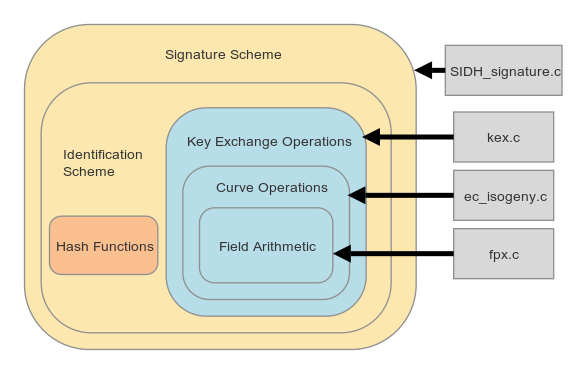
\includegraphics[scale=0.7]{fullmapwcurve.png} % e.g. insert ./image for image.png in the working directory, adjust scale as necessary
\caption{Relationship between SIDH based signatures \& the Yoo et al. fork of the SIDH C library}
\label{fig:fullmap} % insert suitable label, this is used to refer to a fig from within the text as shown above
\end{figure}

\noindent
\emph{Parallelizing Signatures}. Recall now the construction of \textbf{Sign} and \textbf{Verify} from Section \ref{sec:sigsbackground}. The sign procedure requires running $2\lambda$ distinct instances of the underlying key exchange protocol, after which these instances are reproduced in \textbf{Verify} to check for their validity. It is clear that, because every $2\lambda$ iteration of \textbf{Sign} and \textbf{Verify} are entirely independent of each other, these procedures present themselves as embarrassingly parallel.\footnote{in the field of high performance computing, a problem that is trivially parallizable is often referred to as \emph{embarrassingly} parallizable.}

This parallelization approach was exactly the one taken by Yoo et al. in their C implementation. Refer again to the \code{SIDH\_signature.c} functions outlined in Figure \ref{fig:sigfuncs}: \code{isogey\_sign} acts as the entry point for \textbf{Sign} and spawns a POSIX thread for every instance of the procedure's for-loop. So now, in parallel, every thread spawned by \code{isogeny\_sign} makes a call to \code{sign\_thread}, which in turn performs \bob's interaction with \randall. This is illustrated in Figure \ref{fig:parallelcall}. Verification proceeds analogously; \code{isogeny\_verify} is executed and spawns POSIX threads executing \code{verify\_thread} until all $2\lambda$ iterations are complete. $\lambda$ here denotes the security level in bits (128 by default in SIDH), and so 248 threads are spawned in both \code{sign\_thread} and \code{verify\_thread}.

\begin{figure}
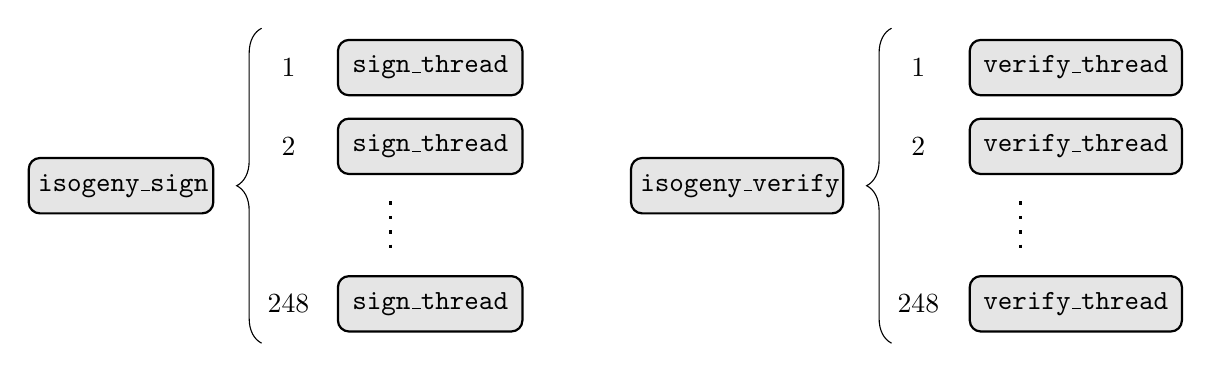
\begin{tikzpicture}
	[scale=1, auto,
		block/.style={
		  rectangle,
		  draw=black,
		  thick,
		  fill=gray!20,
		  text width=6em,
		  align=center,
		  rounded corners,
		  minimum height=2em
		},
		block1/.style={
		  rectangle,
		  draw=black,
		  thick,
		  fill=gray!20,
		  text width=7em,
		  align=center,
		  rounded corners,
		  minimum height=2em
		}
	]
	\begin{scope}[xshift=0cm]
		\draw (2.5,4.5) node[block] {$\code{sign\_thread}$};
		\draw (0.7, 4.5) node {1};
		\draw (2.5,3.5) node[block] {$\code{sign\_thread}$};
		\draw (0.7, 3.5) node {2};
		\draw[very thick, loosely dotted] (2,2.8) -- (2,2.1) node {};
		\draw (2.5,1.5) node[block] {$\code{sign\_thread}$};
		\draw (0.7, 1.5) node {248};

		\draw [decorate,decoration={brace,amplitude=9pt},xshift=-4pt,yshift=0pt] (0.5,1) -- (0.5,5.0) node [black,midway,xshift=-0.6cm,block] {\code{isogeny\_sign}};
	\end{scope}
	\begin{scope}[xshift=8cm]
		\draw (2.7,4.5) node[block1] {$\code{verify\_thread}$};
		\draw (0.7, 4.5) node {1};
		\draw (2.7,3.5) node[block1] {$\code{verify\_thread}$};
		\draw (0.7, 3.5) node {2};
		\draw[very thick, loosely dotted] (2,2.8) -- (2,2.1) node {};
		\draw (2.7,1.5) node[block1] {$\code{verify\_thread}$};
		\draw (0.7, 1.5) node {248};

		\draw [decorate,decoration={brace,amplitude=9pt},xshift=-4pt,yshift=0pt] (0.5,1) -- (0.5,5.0) node [black,midway,xshift=-0.6cm,block1] {\code{isogeny\_verify}};
	\end{scope}
\end{tikzpicture}
\caption{The implementations of \textbf{Sign} and \textbf{Verify}, divided into serial segments \code{isogeny\_sign} and \code{isogeny\_verify} and then parallel segments \code{sign\_thread} and \code{verify\_thread}.}
\label{fig:parallelcall}
\end{figure}

And so, there are two settings in which the same sequence of operations will be carried out $248$ times in parallel. This means that we need only one occurance of an $\mathbb{F}_{p^2}$ inversion in either \code{sign\_thread} or \code{verify\_thread} to be able to fill a element batch of size $248$, suitable for partial batched inversion.

Costello et al. have concisely outlined many of the \sidh isogeny and point-wise functions in Table 1 of \cite{effalg}. Examinig this Figure, we note that there are only three candidate functions containing element inversion calls: \code{j\_inv}, \code{inv\_4\_way}, and \code{get\_A}. The fact that so few functions require inversions is, again, thanks to the design decisions outlined in Section \ref{subsec:design}.\\

\noindent
\code{j\_inv} is a function returning the $j$-invariant of a curve which is used in the derivation of the shared secret. If we refer back to our definitions of \code{Sign} and \code{Verify} (Algorithms 9 and 10, respectively) we note that \code{Sign} contains a call to \code{SecretAgreement\_B} in every iteration of its for-loop. Similarly, \code{Verify} contains a call to \code{SercretAgreement\_A} in roughly half of the iterations of its for-loop, and a call to \code{SecretAgreement\_B} in the remaining iterations. This totals to $248$ secret agreement computations in both signature signing and verifying procedures. This means that somewhere in the exeuction flow of \code{isogney\_sign} and \code{isogeny\_verify} there are calls to these secret agreement functions, illustrating the presence of 1 \code{j\_inv} function call (and by extension, 1 field inversion,) in every signing and verification thread.\\

\noindent
\code{inv\_4\_way} is a function which takes 4 $\mathbb{F}_{p^2}$ elements and returns each elements inversion by means of calculating only one inversion (via the same method outlined by \textbf{BatchedInversion}). This function is used in the key generation to process to invert the Z-values of the public key curve elements; $\phi(P)$, $\phi(Q)$, and $\phi(P-Q)$), so that they can be converted from projective to affine representation. Because every \code{sign\_thread} execution represents \bob's key exchange with a distinct and random \randall, \code{KeyGeneration\_A} must be called in each thread to generate \randall's public and private keys. This results in another candidate batch of size 248 for batched partial inversion.\\

\noindent
\code{get\_A}, while containing an extension field inversion, does not arise in the execution flow of the signature scheme.\\

In Figure \ref{fig:threadcallgraph} we illustrate a heavily simplified call-graph for the \code{sign\_thread} and \code{verify\_thread}, demonstrating where in the execution pipeline \code{j\_inv} and \code{inv\_4\_way} occur. The reader may suspect that, in \code{sign\_thread} for example, the inversions in \code{SecretAgreement\_B} and \code{KeyGeneration\_A} could be batched together to form a batch of 512 elements and to reduce the total number of inversions in \code{isogeny\_sign} to one. This is not possible, however, because the valid execution of \code{SecretAgreement\_B} relies on information returned by \code{KeyGeneration\_A}, and so these inversions must occur sequentially.

\begin{figure}[!h]
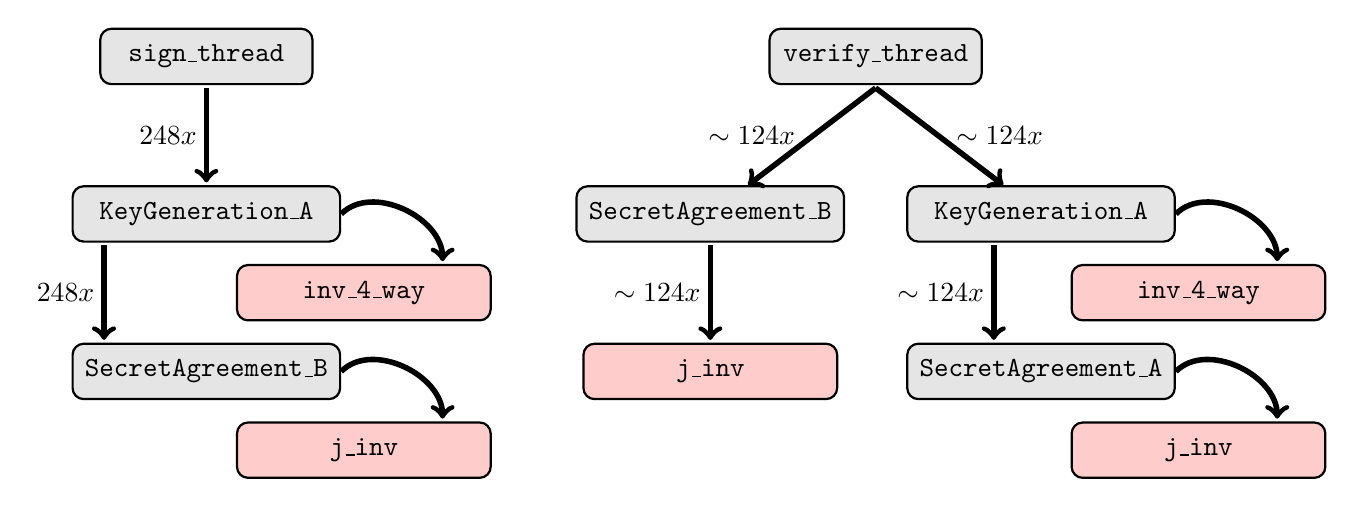
\begin{tikzpicture}
    [auto,
    block/.style={
      rectangle,
      draw=black,
      thick,
      fill=gray!20,
      text width=7em,
      align=center,
      rounded corners,
      minimum height=2em
    },
    block1/.style={
      rectangle,
      draw=black,
      thick,
      fill=gray!20,
      text width=9em,
      align=center,
      rounded corners,
      minimum height=2em
    },
	block2/.style={
      rectangle,
      draw=black,
      thick,
      fill=red!20,
      text width=8.5em,
      align=center,
      rounded corners,
      minimum height=2em
    },
    line/.style={
      draw,thick,
      -latex',
      shorten >=2pt
    },
    cloud/.style={
      draw=red,
      thick,
      ellipse,
      fill=red!20,
      minimum height=1em
    }
  ]
    \draw (1,-2) node[block] (A) {\code{sign\_thread}};
	\draw (9.5,-2) node[block] (B) {\code{verify\_thread}};
    \path (1,-4) node[block1] (C) {\code{KeyGeneration\_A}}
		  (1,-6) node[block1] (D) {\code{SecretAgreement\_B}}
		  (11.6,-4) node[block1] (E) {\code{KeyGeneration\_A}}
          (11.6,-6) node[block1] (F) {\code{SecretAgreement\_A}}
		  (7.4,-4) node[block1] (G) {\code{SecretAgreement\_B}};
	\draw (3,-7) node[block2] (H) {\code{j\_inv}};
	\draw (3,-5) node[block2] (I) {\code{inv\_4\_way}};
	\draw (7.4,-6) node[block2] (J) {\code{j\_inv}};
	\draw (13.6,-5) node[block2] (K) {\code{inv\_4\_way}};
	\draw (13.6,-7) node[block2] (L) {\code{j\_inv}};
	\draw[->, line width=2.0] (1,-2.4) -- (1,-3.6) node[right] {};
		\draw (1, -3) node[left] (LABEL1) {$248x$};
	\draw[->, line width=2.0] (9.5,-2.4) to (E) node[above] {};
		\draw (8.6, -3) node[left] (LABEL4) {$\sim124x$};
	\draw[->, line width=2.0] (9.5,-2.4) to (G) node[right] {};
		\draw (10.4, -3) node[right] (LABEL5) {$\sim124x$};
	\draw[->, line width=2.0] (-0.3,-4.4) -- (-0.3,-5.6) node {};
		\draw (-0.3, -5) node[left] (LABEL6) {$248x$};
	\draw[->, line width=2.0] (7.4,-4.4) -- (7.4,-5.6) node {};
		\draw (7.4, -5) node[left] (LABEL7) {$\sim124x$};
	\draw[->, line width=2.0] (11,-4.4) -- (11,-5.6) node {};
		\draw (11, -5) node[left] (LABEL8) {$\sim124x$};
	\draw[->, line width=2.0] (C.east) to [in=90] (4,-4.6);
	\draw[->, line width=2.0] (D.east) to [in=90] (4,-6.6);
	\draw[->, line width=2.0] (E.east) to [in=90] (14.6,-4.6);
	\draw[->, line width=2.0] (F.east) to [in=90] (14.6,-6.6);

\end{tikzpicture}
\caption{The execution flow of \code{sign\_thread} and \code{verify\_thread} as originally implemented by Yoo et al.}
\label{fig:threadcallgraph}
\end{figure}

To enable batching across execution instances of \code{j\_inv} and \code{inv\_4\_way}, we've supplied new functions \code{j\_inv\_batch} and \code{inv\_4\_way\_batch}. These functions, upon reaching what were originally $\mathbb{F}_{p^2}$ inversions (calls to \code{fp2inv751\_mont}), add their elements that are awaiting inversion to a buffer. Once the buffer of elements has reached its predefined capacity, the final thread to add its element executes \code{pb\_inv} on the buffer. Each thread thereafter, having kept track of where in the buffer they entered their element, retrieves their now inverted element from the buffer returned by \code{pb\_inv}.

\begin{figure}[!h]
\label{fig:batchcallgraph}
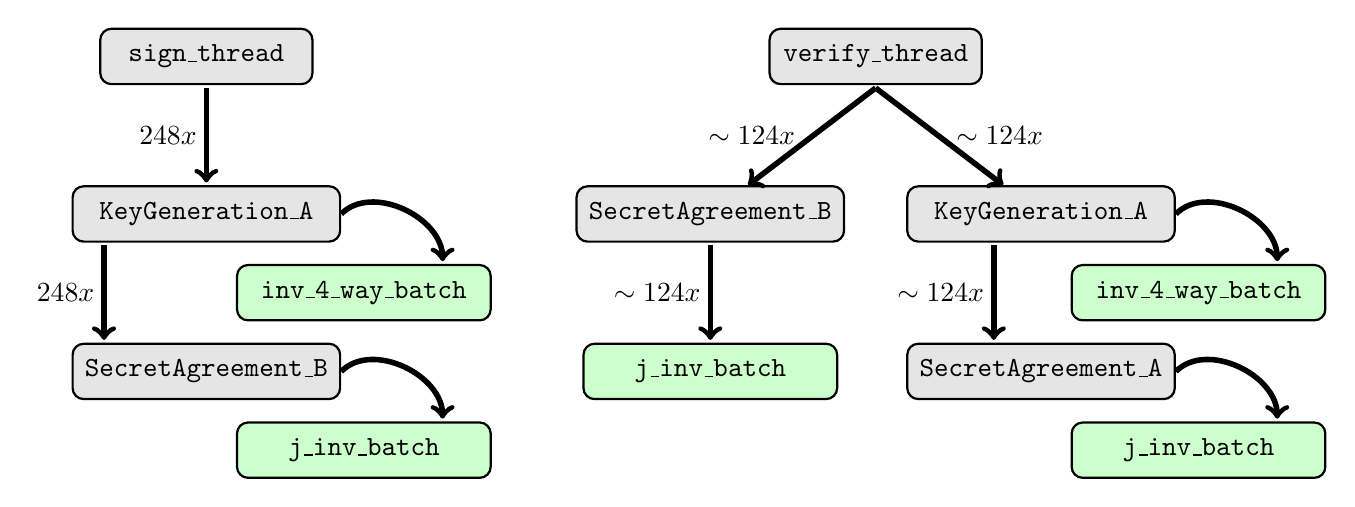
\begin{tikzpicture}
    [auto,
    block/.style={
      rectangle,
      draw=black,
      thick,
      fill=gray!20,
      text width=7em,
      align=center,
      rounded corners,
      minimum height=2em
    },
    block1/.style={
      rectangle,
      draw=black,
      thick,
      fill=gray!20,
      text width=9em,
      align=center,
      rounded corners,
      minimum height=2em
    },
	block2/.style={
      rectangle,
      draw=black,
      thick,
      fill=green!20,
      text width=8.5em,
      align=center,
      rounded corners,
      minimum height=2em
    },
    line/.style={
      draw,thick,
      -latex',
      shorten >=2pt
    },
    cloud/.style={
      draw=red,
      thick,
      ellipse,
      fill=red!20,
      minimum height=1em
    }
  ]

	\draw (1,-2) node[block] (A) {\code{sign\_thread}};
	\draw (9.5,-2) node[block] (B) {\code{verify\_thread}};
	\path (1,-4) node[block1] (C) {\code{KeyGeneration\_A}}
		  (1,-6) node[block1] (D) {\code{SecretAgreement\_B}}
		  (11.6,-4) node[block1] (E) {\code{KeyGeneration\_A}}
		  (11.6,-6) node[block1] (F) {\code{SecretAgreement\_A}}
		  (7.4,-4) node[block1] (G) {\code{SecretAgreement\_B}};
	\draw (3,-7) node[block2] (H) {\code{j\_inv\_batch}};
	\draw (3,-5) node[block2] (I) {\code{inv\_4\_way\_batch}};
	\draw (7.4,-6) node[block2] (J) {\code{j\_inv\_batch}};
	\draw (13.6,-5) node[block2] (K) {\code{inv\_4\_way\_batch}};
	\draw (13.6,-7) node[block2] (L) {\code{j\_inv\_batch}};
	\draw[->, line width=2.0] (1,-2.4) -- (1,-3.6) node[right] {};
		\draw (1, -3) node[left] (LABEL1) {$248x$};
	\draw[->, line width=2.0] (9.5,-2.4) to (E) node[above] {};
		\draw (8.6, -3) node[left] (LABEL4) {$\sim124x$};
	\draw[->, line width=2.0] (9.5,-2.4) to (G) node[right] {};
		\draw (10.4, -3) node[right] (LABEL5) {$\sim124x$};
	\draw[->, line width=2.0] (-0.3,-4.4) -- (-0.3,-5.6) node {};
		\draw (-0.3, -5) node[left] (LABEL6) {$248x$};
	\draw[->, line width=2.0] (7.4,-4.4) -- (7.4,-5.6) node {};
		\draw (7.4, -5) node[left] (LABEL7) {$\sim124x$};
	\draw[->, line width=2.0] (11,-4.4) -- (11,-5.6) node {};
		\draw (11, -5) node[left] (LABEL8) {$\sim124x$};
	\draw[->, line width=2.0] (C.east) to [in=90] (4,-4.6);
	\draw[->, line width=2.0] (D.east) to [in=90] (4,-6.6);
	\draw[->, line width=2.0] (E.east) to [in=90] (14.6,-4.6);
	\draw[->, line width=2.0] (F.east) to [in=90] (14.6,-6.6);

\end{tikzpicture}
\caption{The execution flow of \code{sign\_thread} and \code{verify\_thread} when run with inversion batching enabled}
\end{figure}

To properly implement \code{pb\_inv} in these functions, we modify every function along the call stack leading up to \code{j\_inv} and \code{inv\_4\_way}: \code{SecretAgreement\_A}, \code{SecretAgreement\_B}, and \code{KeyGeneration\_A}. Our modifications allow these functions to optionally pass a C struct we've defined which holds all of the information necessary for a successfull execution of \code{pb\_inv}. We refer to this structure as \code{batch\_struct}, and it holds the following: an integer \code{batchSize} denoting the number of elements in the batch, an integer \code{cntr} which tracks how many elements are currently in the batch (and is invariably less than or equal to \code{batchSize}), an \code{f2elm\_t} buffer \code{invArray} for storing the elements to be inverted, and an \code{f2elm\_t} buffer \code{invDest} for storing the inversion results.

Once one of the aforementioned \code{kex.c} functions reaches its call to either \code{j\_inv} or \code{inv\_4\_way}, the function checks whether the \code{batch\_struct} it has been passed is \code{NULL}. If the \code{batch\_struct} is defined, the call to \code{j\_inv} or \code{inv\_4\_way} is replaced with a call to \code{j\_inv\_batch} or \code{inv\_4\_way\_batch}, respectively.

A mutex lock can also be found in the \code{batch\_struct}, allowing \code{j\_inv} and \code{inv\_4\_way} to increment the size of the batch safely across threads. Each thread performs the following as it approaches the inversion call:
\begin{enumerate}
\item acquire the mutex lock
\item add element to be inverted to \code{invArray}
\item store the current value of \code{cntr} locally
\item increment \code{cntr}
\item release the lock
\end{enumerate}

A semaphore has also been included in \code{batch\_struct}, the function of which is to ensure that each thread knows to wait until the batch has been filled (248 elements in the signing case, ~128 in the verification cases) before it attempts to access its inverted element. If the locally stored \code{cntr} is less than \code{batchSize}, the current thread waits on the semaphore. If the locally stored \code{cntr} is equal to \code{batchSize}, this implies the current thread is the last to add its element - this thread then carries out execution of \code{pb\_inv} and upon completion posts the sempahore. After the semaphore has been posted, all other threads are able to resume execution and retrieve their now inverted elements.\\

\begin{center}
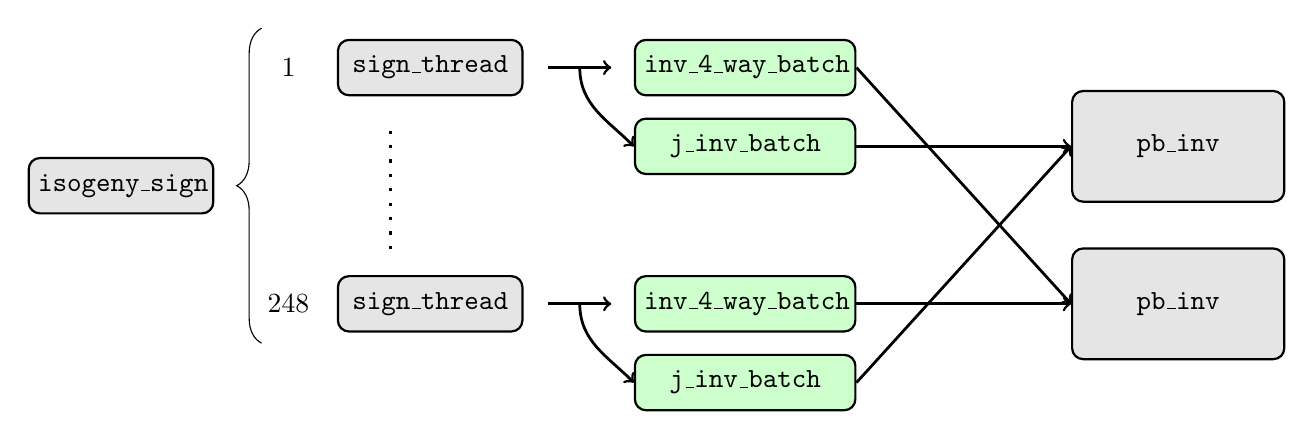
\begin{tikzpicture}
	[scale=1, auto,
		block/.style={
		  rectangle,
		  draw=black,
		  thick,
		  fill=gray!20,
		  text width=6em,
		  align=center,
		  rounded corners,
		  minimum height=2em
		},
		blockgreen/.style={
		  rectangle,
		  draw=black,
		  thick,
		  fill=green!20,
		  text width=7.3em,
		  align=center,
		  rounded corners,
		  minimum height=2em
		},
		batchblock/.style={
		  rectangle,
		  draw=black,
		  thick,
		  fill=gray!20,
		  text width=7em,
		  align=center,
		  rounded corners,
		  minimum height=4em
		}
	]
	\draw (2.5,4.5) node[block] {\code{sign\_thread}};
	\draw[->, line width=1.0] (4,4.5) -- (4.8,4.5) node {};
	%\draw [decorate,decoration={brace,amplitude=9pt},xshift=-4pt,yshift=0pt] (4.7,3.2) -- (4.7,5.7) node [black,midway,xshift=-0.6cm,block] {\code{sign\_thread}};
	\draw (6.5,3.5) node[blockgreen] (JINV1) {\code{j\_inv\_batch}};
	\draw (6.5,4.5) node[blockgreen] (INV1) {\code{inv\_4\_way\_batch}};
	\draw (0.7, 4.5) node {1};

	\draw[very thick, loosely dotted] (2,3.7) -- (2,2.2) node {};

	\draw (2.5,1.5) node[block] {\code{sign\_thread}};
	\draw[->, line width=1.0] (4,1.5) -- (4.8,1.5) node {};
	%\draw [decorate,decoration={brace,amplitude=9pt},xshift=-4pt,yshift=0pt] (4.7,0.3) -- (4.7,2.8) node [black,midway,xshift=-0.6cm,block] {\code{sign\_thread}};
	\draw (6.5,0.5) node[blockgreen] (JINV2) {\code{j\_inv\_batch}};
	\draw (6.5,1.5) node[blockgreen] (INV2) {\code{inv\_4\_way\_batch}};
	\draw (0.7, 1.5) node {248};

	\draw[->, line width=1.0] (4.4,4.5) to [out=-90] (JINV1.west);
	\draw[->, line width=1.0] (4.4,1.5) to [out=-90] (JINV2.west);

	\draw [decorate,decoration={brace,amplitude=9pt},xshift=-4pt,yshift=0pt] (0.5,1) -- (0.5,5.0) node [black,midway,xshift=-0.6cm,block] {\code{isogeny\_sign}};

	\draw (12,3.5) node[batchblock] (BATCH1) {\code{pb\_inv}};
	\draw (12,1.5) node[batchblock] (BATCH2) {\code{pb\_inv}};

	\draw[->, line width=1.0] (JINV1.east) to (BATCH1.west) node {};
	\draw[->, line width=1.0] (JINV2.east) to (BATCH1.west) node {};
	\draw[->, line width=1.0] (INV1.east) to (BATCH2.west) node {};
	\draw[->, line width=1.0] (INV2.east) to (BATCH2.west) node {};
\end{tikzpicture}
\end{center}

C code for all of these functions (with comparable differences highlighted) can be found in Appendix \ref{app:functions}.

\section{Results}

Our results come in several forms. First, there are the execution-time results of \code{pb\_inv}, compared with plain batching and unbatched inversions. Measurements of this first type are gathered in a general $\mathbb{F}_{p^2}$ environment constructed using the NTL C++ library. This allows us to meaure how the performance of \code{pb\_inv} compares with other approaches for arbitrarily sized moduli. These numbers can be found in Figures \ref{fig:moduli100} and \ref{fig:moduli1000}, and are measured in seconds. The benchmarks were taken on a single-core 1.3GHz AMD processor.

\begin{figure}[!h]
\begin{center}
\begin{tabular}{@{}llll@{}}
	\toprule
	Modulus Size & Regular Batch & \code{pb\_inv} & Unbatched \\
	\midrule
	32 & 0.351996 & 0.13946 & 0.159744\\
	64 & 0.335376 & 0.132932 & 0.167551\\
	128 & 0.356995 & 0.150744 & 0.299575\\
	256 & 0.748303 & 0.207973 & 0.486726\\
	512 & 0.655977 & 0.34409 & 0.886866\\
	1024 & 1.49688 & 0.762736 & 1.83442\\
	2048 & 3.44086 & 2.07405 & 4.39554\\
	\bottomrule
\end{tabular}
\end{center}
\caption{Execution time in seconds for 100 field element inversions using various techniques and modulus sizes (measured in seconds)}
\label{fig:moduli100}
\end{figure}

\begin{figure}[!h]
\begin{center}
\begin{tabular}{@{}llll@{}}
	\toprule
	Modulus Size & Regular Batch & \code{pb\_inv} & Unbatched \\
	\midrule
	32 & 3.45507 & 1.35421 & 1.51127\\
	64 & 3.4481 & 1.32611 & 1.61707\\
	128 & 3.64458 & 1.54956 & 2.95078\\
	256 & 7.00599 & 2.18369 & 4.80218\\
	512 & 6.563 & 3.39861 & 8.87935\\
	1024 & 14.8953 & 7.90045 & 18.3234\\
	2048 & 36.216 & 22.2085 & 42.616\\
	\bottomrule
\end{tabular}
\end{center}
\caption{Execution time in seconds for 1000 field element inversions using various techniques and modulus sizes (measured in seconds)}
\label{fig:moduli1000}
\end{figure}

The reader will note that the scale factor on performance as modulus size increases is significantly lower for \code{pb\_inv} than it is for other approaches. This is important because, as the computational power of adversaries increases, modulus sizes increase in order to ensure that compromising secret keys via a brute-force attack remains adequately difficult.

Also worth noting is how the non-partial batching algorithm performs poorly when the modulus is small. This could be an indication that for small modulus N, multiplications quickly approach the computational cost of inversions for extension field elements.\\

\noindent
We also measure the improvement in the performance of signature signing and verifying procedures offered by the inclusion of the batched partial inversion mechanism. Figure \ref{fig:batchgains} provides benchmarks for KeyGen, Sign, and Verify procedures with both batched partial inversion implemented (in the previously mentioned locations) and not implemented. All benchmarks are averages computed from 100 randomized sample runs. These results are measured in clock cycles and run on a quad-core Intel i5-8250U 1.6GHz processor.\\

\begin{figure}
\begin{center}
\begin{tabular}{@{}lllll@{}}
	\toprule
	Procedure & Without Batching & With Batching\\
	\midrule
	KeyGen & 84,499,270 & 84,499,270\\
	Signature Sign & 4,950,023,141.65 & 4,552,062,482.520\\
	Signature Verify & 3,466,703,991.09 & 3,173,340,239.461\\
	\bottomrule
\end{tabular}
\end{center}
\caption{Performance comparisons of signature subroutines run with and without batching.}
\label{fig:batchgains}
\end{figure}

With inversion batching turned on we notice a ${\sim}8$\% performance increase for both signature signing and verification.\\

\chapter{Compressing Signatures}
\label{sec:compress}

Our second contribution, also in the form of an addendum to the \sidh signature extension, is a mechanism for compressing signatures to reduce the size.

Costello et al. showed in \cite{pkcomp} that  

\section{SIDH Key Compression Background}

We discussed rejection sampling A values from signature public keys until we found an A that was also the x-coord of a point. After some simple analysis, however, we found that it was extremely unlikely for A to be a point on the curve.

\subsection{Construction of Bases}

\subsection{Pohlig-Hellman}

\subsection{Decompression}

\section{Implementation Details}

\subsection{Tailoring Compression for Signatures}

\subsection{Decompressing $\psi(S)$}

\section{Results}

Our technique can reduce the size of \sidh signature compression from \_\_\_ bits to \_\_\_ bits.

\subsection{Analysis}

\subsection{Potential Performance Improvements}


\chapter{Discussion \& Conclusion}

\section{Results \& Comparisons}

\subsection{Combining Batching \& Compression}

\begin{center}
\begin{tabular}{l | b | b | b }
\hline
\mc{1}{}  & \mc{1}{Key Gen} & \mc{1}{Sign} & \mc{1}{Verify}\\
\hline
\rowcolor{Gray}
SIDH & a & b & c \\
Sphincs & a & b & c \\
Rainbow & a & b & c \\
qTESLA & a & b & c \\
Picnic & a & b & c \\
\rowcolor{light-red}
RSA & a & b & c \\
\rowcolor{light-red}
ECDSA & a & b & c \\
\hline
\end{tabular}
\end{center}

\begin{center}
\begin{tabular}{l | b | b | b }
\hline
\mc{1}{}  & \mc{1}{Public Key} & \mc{1}{Private Key} & \mc{1}{Signature}\\
\hline
\rowcolor{Gray}
SIDH & 768 & b & 141,312 \\
Sphincs & 32 & 64 & 8,080 - 16,976 \\
Rainbow & 152,097 - 192,241 & 100,209 - 114,308 & 64 - 104 \\
qTESLA & 4,128 & 2,112 & 3,104 \\
Picnic & 33 & 49 & 34,004 - 53,933 \\
\rowcolor{light-red}
RSA & 384 & b & 384 \\
\rowcolor{light-red}
ECDSA & 32 & b & 32 \\
\hline
\end{tabular}
\end{center}

\section{Additional Opportunities for Batching}
\label{sec:morebatch}

\section{Future Work}

\begin{appendices}
	\chapter{\sidh Functions}
\label{app:functions}

\section{$\mathbb{F}_p$ and $\mathbb{F}_{p^2}$ Functions}

\section{Isogeny and Point-wise Functions}

\subsection{\code{j\_inv}}

\begin{lstlisting}[basicstyle=\tiny]
void j_inv(const f2elm_t A, const f2elm_t C, f2elm_t jinv) {
	f2elm_t t0, t1;
	fp2sqr751_mont(A, jinv);                           // jinv = A^2
	fp2sqr751_mont(C, t1);                             // t1 = C^2
	fp2add751(t1, t1, t0);                             // t0 = t1+t1
	fp2sub751(jinv, t0, t0);                           // t0 = jinv-t0
	fp2sub751(t0, t1, t0);                             // t0 = t0-t1
	fp2sub751(t0, t1, jinv);                           // jinv = t0-t1
	fp2sqr751_mont(t1, t1);                            // t1 = t1^2
	fp2mul751_mont(jinv, t1, jinv);                    // jinv = jinv*t1
	fp2add751(t0, t0, t0);                             // t0 = t0+t0
	fp2add751(t0, t0, t0);                             // t0 = t0+t0
	fp2sqr751_mont(t0, t1);                            // t1 = t0^2
	fp2mul751_mont(t0, t1, t0);                        // t0 = t0*t1
	fp2add751(t0, t0, t0);                             // t0 = t0+t0
	fp2add751(t0, t0, t0);                             // t0 = t0+t0
	fp2inv751_mont(jinv);                              // jinv = 1/jinv
	fp2mul751_mont(jinv, t0, jinv);                    // jinv = t0*jinv
}
\end{lstlisting}

\subsection{\code{j\_inv\_batch}}

\begin{lstlisting}[basicstyle=\tiny]
void j_inv_batch(f2elm_t A, f2elm_t C, f2elm_t jinv, invBatch* batch) {
	f2elm_t t0, t1;
\end{lstlisting}
\vspace{-0.75\baselineskip}
\begin{lstlisting}[backgroundcolor=\color{light-green}, firstnumber=3, basicstyle=\tiny]
	int tempCnt;
\end{lstlisting}
\vspace{-0.75\baselineskip}
\begin{lstlisting}[firstnumber=4, basicstyle=\tiny]
	fp2sqr751_mont(A, jinv);                           // jinv = A^2
	fp2sqr751_mont(C, t1);                             // t1 = C^2
	fp2add751(t1, t1, t0);                             // t0 = t1+t1
	fp2sub751(jinv, t0, t0);                           // t0 = jinv-t0
	fp2sub751(t0, t1, t0);                             // t0 = t0-t1
	fp2sub751(t0, t1, jinv);                           // jinv = t0-t1
	fp2sqr751_mont(t1, t1);                            // t1 = t1^2
	fp2mul751_mont(jinv, t1, jinv);                    // jinv = jinv*t1
	fp2add751(t0, t0, t0);                             // t0 = t0+t0
	fp2add751(t0, t0, t0);                             // t0 = t0+t0
	fp2sqr751_mont(t0, t1);                            // t1 = t0^2
	fp2mul751_mont(t0, t1, t0);                        // t0 = t0*t1
	fp2add751(t0, t0, t0);                             // t0 = t0+t0
	fp2add751(t0, t0, t0);                             // t0 = t0+t0
\end{lstlisting}
\vspace{-0.75\baselineskip}
\begin{lstlisting}[backgroundcolor=\color{light-green}, firstnumber=19, basicstyle=\tiny]
	pthread_mutex_lock(&batch->arrayLock);
	fp2copy751(jinv, batch->invArray[batch->cntr]);
	tempCnt = batch->cntr;
	batch->cntr++;
	pthread_mutex_unlock(&batch->arrayLock);

	int i;
	if (tempCnt+1 == batch->batchSize) {
		partial_batched_inv(batch->invArray, batch->invDest, batch->batchSize);
		for (i = 0; i < batch->batchSize - 1; i++) {
			sem_post(&batch->sign_sem);
		}
	} else {
		sem_wait(&batch->sign_sem);
	}
	fp2copy751(batch->invDest[tempCnt], jinv);
	batch->cntr = 0;
\end{lstlisting}%
\vspace{-0.75\baselineskip}
\begin{lstlisting}[firstnumber=36, basicstyle=\tiny]
	fp2mul751_mont(jinv, t0, jinv);                    // jinv = t0*jinv
}
\end{lstlisting}

\subsection{\code{inv\_4\_way}}

\begin{lstlisting}[basicstyle=\tiny]
void inv_4_way(f2elm_t z1, f2elm_t z2, f2elm_t z3, f2elm_t z4) {
  	f2elm_t t0, t1, t2;
	int tempCnt;

    fp2mul751_mont(z1, z2, t0);                      // t0 = z1*z2
    fp2mul751_mont(z3, z4, t1);                      // t1 = z3*z4
    fp2mul751_mont(t0, t1, t2);                      // t2 = z1*z2*z3*z4
    fp2inv751_mont(t2);                              // t2 = 1/(z1*z2*z3*z4)
    fp2mul751_mont(t0, t2, t0);                      // t0 = 1/(z3*z4)
    fp2mul751_mont(t1, t2, t1);                      // t1 = 1/(z1*z2)
    fp2mul751_mont(t0, z3, t2);                      // t2 = 1/z4
    fp2mul751_mont(t0, z4, z3);                      // z3 = 1/z3
    fp2copy751(t2, z4);                              // z4 = 1/z4
    fp2mul751_mont(z1, t1, t2);                      // t2 = 1/z2
    fp2mul751_mont(z2, t1, z1);                      // z1 = 1/z1
    fp2copy751(t2, z2);                              // z2 = 1/z2
}
\end{lstlisting}

\subsection{\code{inv\_4\_way\_batch}}

\begin{lstlisting}[basicstyle=\tiny,]
void inv_4_way_batch(f2elm_t z1, f2elm_t z2, f2elm_t z3, f2elm_t z4, invBatch* batch) {
  	f2elm_t t0, t1, t2;
	int tempCnt;

    fp2mul751_mont(z1, z2, t0);                      // t0 = z1*z2
    fp2mul751_mont(z3, z4, t1);                      // t1 = z3*z4
    fp2mul751_mont(t0, t1, t2);                      // t2 = z1*z2*z3*z4
\end{lstlisting}
\vspace{-0.75\baselineskip}
\begin{lstlisting}[backgroundcolor = \color{light-green}, firstnumber=8, basicstyle=\tiny]
	pthread_mutex_lock(&batch->arrayLock);
	fp2copy751(t2, batch->invArray[batch->cntr]);
	tempCnt = batch->cntr;
	batch->cntr++;
	pthread_mutex_unlock(&batch->arrayLock);
	int i;
	if (tempCnt+1 == batch->batchSize) {
		partial_batched_inv(batch->invArray, batch->invDest, batch->batchSize);
		for (i = 0; i < batch->batchSize; i++) {
			sem_post(&batch->sign_sem);
		}
	} else {
		sem_wait(&batch->sign_sem);
	}
	fp2copy751(batch->invDest[tempCnt], t2);
	batch->cntr = 0;
\end{lstlisting}
\vspace{-0.9\baselineskip}
\begin{lstlisting}[firstnumber=24,basicstyle=\tiny]
    fp2mul751_mont(t0, t2, t0);                      // t0 = 1/(z3*z4)
    fp2mul751_mont(t1, t2, t1);                      // t1 = 1/(z1*z2)
    fp2mul751_mont(t0, z3, t2);                      // t2 = 1/z4
    fp2mul751_mont(t0, z4, z3);                      // z3 = 1/z3
    fp2copy751(t2, z4);                              // z4 = 1/z4
    fp2mul751_mont(z1, t1, t2);                      // t2 = 1/z2
    fp2mul751_mont(z2, t1, z1);                      // z1 = 1/z1
    fp2copy751(t2, z2);                              // z2 = 1/z2
}
\end{lstlisting}

\section{Key Exchange Functions}

\begin{lstlisting}[basicstyle=\tiny,]
CRYPTO_STATUS KeyGeneration_A(unsigned char* pPrivateKeyA,
                              unsigned char* pPublicKeyA,
							  PCurveIsogenyStruct CurveIsogeny,
							  bool GenerateRandom, batch_struct* batch) {
	unsigned int owords = NBITS_TO_NWORDS(CurveIsogeny->owordbits);
	unsigned int pwords = NBITS_TO_NWORDS(CurveIsogeny->pwordbits);
	point_basefield_t P;
	point_proj_t R, phiP = {0}, phiQ = {0}, phiD = {0};
  point_proj_t pts[MAX_INT_POINTS_ALICE];
	publickey_t* PublicKeyA = (publickey_t*)pPublicKeyA;
	unsigned int i, row, m, index = 0, npts = 0;
  unsigned int pts_index[MAX_INT_POINTS_ALICE];
	f2elm_t coeff[5], A = {0}, C = {0}, Aout, Cout;
	CRYPTO_STATUS Status = CRYPTO_ERROR_UNKNOWN;

	if (pPrivateKeyA == NULL ||
         pPublicKeyA == NULL  ||
         is_CurveIsogenyStruct_null(CurveIsogeny)) {
		return CRYPTO_ERROR_INVALID_PARAMETER;
	}

	if (GenerateRandom) {
		Status = random_mod_order((digit_t*)pPrivateKeyA, ALICE, CurveIsogeny);
		if (Status != CRYPTO_SUCCESS) {
			clear_words((void*)pPrivateKeyA, owords);
			return Status;
		}
	}

	to_mont((digit_t*)CurveIsogeny->PA, (digit_t*)P);
	to_mont(((digit_t*)CurveIsogeny->PA)+NWORDS_FIELD, ((digit_t*)P)+NWORDS_FIELD);

	Status = secret_pt(P, (digit_t*)pPrivateKeyA, ALICE, R, CurveIsogeny);
	if (Status != CRYPTO_SUCCESS) {
		clear_words((void*)pPrivateKeyA, owords);
		return Status;
	}

	copy_words((digit_t*)CurveIsogeny->PB, (digit_t*)phiP, pwords);
	fpcopy751((digit_t*)CurveIsogeny->Montgomery_one, (digit_t*)phiP->Z);
	to_mont((digit_t*)phiP, (digit_t*)phiP);
	copy_words((digit_t*)phiP, (digit_t*)phiQ, pwords);
	fpneg751(phiQ->X[0]);
	fpcopy751((digit_t*)CurveIsogeny->Montgomery_one, (digit_t*)phiQ->Z);
	distort_and_diff(phiP->X[0], phiD, CurveIsogeny);

	fpcopy751(CurveIsogeny->A, A[0]);
	fpcopy751(CurveIsogeny->C, C[0]);
	to_mont(A[0], A[0]);
	to_mont(C[0], C[0]);

	first_4_isog(phiP, A, Aout, Cout, CurveIsogeny);
	first_4_isog(phiQ, A, Aout, Cout, CurveIsogeny);
	first_4_isog(phiD, A, Aout, Cout, CurveIsogeny);
	first_4_isog(R, A, A, C, CurveIsogeny);

	index = 0;
	for (row = 1; row < MAX_Alice; row++) {
		while (index < MAX_Alice-row) {
			fp2copy751(R->X, pts[npts]->X);
			fp2copy751(R->Z, pts[npts]->Z);
			pts_index[npts] = index;
			npts += 1;
			m = splits_Alice[MAX_Alice-index-row];
			xDBLe(R, R, A, C, (int)(2*m));
			index += m;
		}
		get_4_isog(R, A, C, coeff);

		for (i = 0; i < npts; i++) {
			eval_4_isog(pts[i], coeff);
		}
		eval_4_isog(phiP, coeff);
		eval_4_isog(phiQ, coeff);
		eval_4_isog(phiD, coeff);

		fp2copy751(pts[npts-1]->X, R->X);
		fp2copy751(pts[npts-1]->Z, R->Z);
		index = pts_index[npts-1];
		npts -= 1;
	}

	get_4_isog(R, A, C, coeff);
	eval_4_isog(phiP, coeff);
	eval_4_isog(phiQ, coeff);
	eval_4_isog(phiD, coeff);

	if(batch != NULL) {
		inv_4_way_batch(C, phiP->Z, phiQ->Z, phiD->Z, batch);
	} else {
		inv_4_way(C, phiP->Z, phiQ->Z, phiD->Z);
	}

	fp2mul751_mont(A, C, A);
	fp2mul751_mont(phiP->X, phiP->Z, phiP->X);
	fp2mul751_mont(phiQ->X, phiQ->Z, phiQ->X);
	fp2mul751_mont(phiD->X, phiD->Z, phiD->X);

	from_fp2mont(A, ((f2elm_t*)PublicKeyA)[0]);
	from_fp2mont(phiP->X, ((f2elm_t*)PublicKeyA)[1]);
	from_fp2mont(phiQ->X, ((f2elm_t*)PublicKeyA)[2]);
	from_fp2mont(phiD->X, ((f2elm_t*)PublicKeyA)[3]);

	clear_words((void*)R, 2*2*pwords);
	clear_words((void*)phiP, 2*2*pwords);
	clear_words((void*)phiQ, 2*2*pwords);
	clear_words((void*)phiD, 2*2*pwords);
	clear_words((void*)pts, MAX_INT_POINTS_ALICE*2*2*pwords);
	clear_words((void*)A, 2*pwords);
	clear_words((void*)C, 2*pwords);
	clear_words((void*)coeff, 5*2*pwords);

	return Status;
}
\end{lstlisting}

\end{appendices}
\cleardoublepage
%\pagebreak
\phantomsection


\bibliographystyle{alphaurl}
\bibliography{refs.bib, abbrev3, crypto}


\end{document}
